\documentclass{egpubl}
\JournalSubmission

\usepackage[T1]{fontenc}
\usepackage{dfadobe}
\usepackage{cite}
\BibtexOrBiblatex
\electronicVersion
\PrintedOrElectronic
\ifpdf \usepackage[pdftex]{graphicx} \pdfcompresslevel=9
\else \usepackage[dvips]{graphicx} \fi
\usepackage{egweblnk}

\usepackage{amsmath,amssymb}
% egpubl defines its own proof environment, which amsthm then refuses to
% redefine; ceding it to amsthm keeps the Guarantees section's proofs working.
\let\proof\relax
\let\endproof\relax
\usepackage{amsthm}
\usepackage{booktabs}
\usepackage{microtype}
\usepackage{algorithm}
\usepackage{algpseudocode}

\graphicspath{{../figures/}}

\newtheorem{proposition}{Proposition}
\newtheorem{corollary}[proposition]{Corollary}
\theoremstyle{definition}
\newtheorem{remark}[proposition]{Remark}

\newcommand{\R}{\mathbb{R}}
\newcommand{\lab}{\ell}
\newcommand{\labels}{\mathcal{K}}
\newcommand{\tet}{\tau}
\newcommand{\interp}{F}
\newcommand{\region}[1]{R_{#1}}
\newcommand{\dregion}[1]{\widehat{R}_{#1}}

\title[Exact Differentiable Extraction of Multi-Material Interfaces]%
      {Exact Differentiable Extraction of Multi-Material Interfaces}

\author[M. Ozlem]{Melih Ozlem\\ AI Science Research\\ Mountain View, CA, USA\\ \texttt{aiscienceresearch.com}\\ \texttt{melih.ozlem@aiscienceresearch.com}}

\begin{document}
\maketitle

\begin{abstract}
Differentiable isosurface extraction bridges implicit geometry and
gradient-based optimisation, but every method in use is two-label.
Multi-material geometry differs in kind: triple curves and quadruple points
have no two-label analogue, and the strongest differentiable extractors
guarantee two-manifold output, which is precisely what a triple curve
violates. Robust arrangement algorithms do compute the exact argmax partition
of a piecewise-linear multi-label field, but encode vertices implicitly and
resolve them with exact predicates --- the source of their robustness and the
reason no derivative survives.
We obtain the same partition on a conforming tetrahedral grid from small
closed-form linear solves instead, so a vertex is an explicit differentiable
function of the nodal logits and ordinary reverse-mode autograd supplies exact
gradients, at the cost of replacing exact predicates with a symbolic
perturbation. That cost is measured, not argued: on identical tetrahedra our
output matches the reference implementation of the exact construction to
$10^{-14}$, differing only where coincidences make the arrangement itself
ambiguous. A power-diagram cell is recovered to $2.5\times10^{-16}$ relative
error in volume and area. Against the strongest differentiable extractor we are
more accurate at extracting a known two-label field and less accurate at
optimising one, while its route to three regions, extracting each against the
rest, returns no partition at any resolution tried. Minimising interface area
at equal volumes in 3D recovers the standard double bubble, while corner-label
case analysis, the obvious multi-label generalisation, settles on a different
shape; both minimisers lie inside the
representable family, so this tests the gradient path, not the representation.
Because the partition cannot represent interpenetration, the same operator
makes contact between solid objects differentiable: the shared surface is
emitted once rather than as two coincident sheets, and a loss reading only
those patches drives three prescribed contact areas, reachable by construction,
to $6.5\times10^{-5}$ relative error with no penalty term.

\begin{CCSXML}
<ccs2012>
<concept>
<concept_id>10010147.10010371.10010396.10010397</concept_id>
<concept_desc>Computing methodologies~Mesh geometry models</concept_desc>
<concept_significance>500</concept_significance>
</concept>
<concept>
<concept_id>10010147.10010371.10010396.10010402</concept_id>
<concept_desc>Computing methodologies~Shape modeling</concept_desc>
<concept_significance>300</concept_significance>
</concept>
<concept>
<concept_id>10002950.10003714.10003715.10003750</concept_id>
<concept_desc>Mathematics of computing~Mesh generation</concept_desc>
<concept_significance>300</concept_significance>
</concept>
</ccs2012>
\end{CCSXML}

\ccsdesc[500]{Computing methodologies~Mesh geometry models}
\ccsdesc[300]{Computing methodologies~Shape modeling}
\ccsdesc[300]{Mathematics of computing~Mesh generation}

\printccsdesc
\end{abstract}


\section{Introduction}
\label{sec:intro}

An implicit representation stores geometry as a function rather than a
mesh~\cite{park2019, mescheder2019}, and most downstream machinery wants the
mesh back. When the function is being optimised the conversion has to be
differentiable, which is why a line of work from Deep Marching
Cubes~\cite{liao2018} through MeshSDF~\cite{remelli2020}, DMTet~\cite{shen2021}
and FlexiCubes~\cite{shen2023} has made isosurface extraction into a
differentiable operator.

All of it is two-label: the input is a scalar field and the output separates its
sub-level set from its super-level set. A great deal of geometry is not like
that. A segmented medical image assigns one of several tissue labels to each
voxel; a composite part is a partition into materials; a grain structure is a
partition into crystals. What makes these different is not that there are more
surfaces but that there are new kinds of feature: three regions meet along a
curve and four at isolated points, which is where a two-label method has nothing
to say, because with two labels such features cannot occur.

Two lineages bear on this and their intersection is empty. The multi-material
extraction literature adopts our exact model --- per-label values at the grid
nodes, interpolated and then argmaxed --- as far back as Hege et
al.~\cite{hege1997}, who state it, approximate it by subsampling because they
cannot solve it, and promise the general case in a paper that never followed;
much of what they left behind is what CGAL ships today~\cite{cgalmesh3}. The
exact computation did arrive, in Du et al.~\cite{du2022}, which partitions each
tetrahedron of a piecewise-linear multi-label field correctly for any number of
labels and recovers the whole non-manifold structure --- by encoding vertices
implicitly and resolving them with exact predicates, a construction no
derivative survives. The differentiable lineage has derivatives but is two-label
by construction, and its strongest members guarantee two-manifold
output~\cite{shen2023, tetweave2025}, which is exactly what a triple curve
violates. A third community, interface reconstruction for multi-material
hydrodynamics, reaches the same junctions from volume fractions and reports the
same obstruction. Section~\ref{sec:related} traces all three. What is missing is
not the partition but a path for gradients through it, and that is the operator
described here.

One pipeline makes the shape of the gap concrete. Rule-based cardiac fibre
generation assigns a myocyte orientation to every point of a ventricular mesh
from the gradients of a few Laplace--Dirichlet solutions~\cite{bayer2012}, and
its extension to outflow tracts needs each valve as a separately identified
surface~\cite{doste2019}: the labels on the interfaces \emph{are} the Dirichlet
boundaries~\cite{svmultiphysics}. What is available instead is a chain ---
extract each boundary, smooth the staircase, merge, tetrahedralise, recover
which region is which from seed points --- in which every step can let the
labelling drift out of agreement with the geometry, and which has no derivative
end to end. We offer this as motivation rather than result:
Section~\ref{sec:realdata} shows the operator meets that input contract on
clinical segmentation output, but we do not run the fibre computation.
\medskip
\noindent This paper contributes:

\begin{enumerate}
\item \textbf{A negative result with a measurement.} Per-cell corner-label case
analysis --- the mechanism behind marching cubes and its multi-material
descendants~\cite{lorensen1987, hege1997} --- is not merely inaccurate in 3D but
wrong at a rate that stays near one half and does not approach zero under
refinement, on both fields we measured (Section~\ref{sec:failure}).
That label-separating methods miss structure the grid does not resolve is
observed qualitatively by Du et al.~\cite{du2022}; what we add is the geometric
reason and the rate.

\item \textbf{A differentiable route to the exact arrangement.} We extract the
exact arrangement of the piecewise-linear interpolant of the logits
(Section~\ref{sec:method}), which Du et al.~\cite{du2022} already compute, but
by a different means and for a different purpose. Every vertex is a small
closed-form linear solve keyed by \emph{label set} rather than by cell, so its
position is an explicit differentiable function of the nodal logits rather than
an implicit encoding decided by a predicate. Keying by label set also lets one
cell carry several features, which a case table cannot name.

\item \textbf{Guarantees instead of heuristics} (Section~\ref{sec:guarantees}):
convexity of patches, exactness on affine logits and hence on power diagrams,
and conformity across cells without a welding step; closure and orientability
of each region are checked rather than proved, as are dihedral angles landing
within $0.4^\circ$ of $120^\circ$ on a curved interface. These are validated
against closed-form ground truth by $52$ automated checks in 2D and 3D, all
passing, and against the one implementation computing the same partition, that
of Du et al.~\cite{du2022}: given identical tetrahedra, the two agree vertex
for vertex and patch for patch to $10^{-14}$ on all eight configurations we ran
whose answer is unique, the largest being $663\,552$ tetrahedra of clinical
segmentation output (Section~\ref{sec:headtohead}). Against
FlexiCubes~\cite{shen2023}, the differentiable extractor the construction
claims to subsume, we extract a known field more accurately, optimise one less
accurately, and return a partition of three regions where its one-vs-rest
output is not one at any resolution (Section~\ref{sec:flexicubes}).

\item \textbf{Optimisation through a 3D triple curve}
(Section~\ref{sec:doublebubble}): minimising interface area at equal volumes
recovers the standard double bubble, with $r_1/d = r_2/d = 1.0064$ against the
exact $1$ and dihedral angles within $0.4^\circ$ of $120^\circ$, converging at
second order. Substituting corner-label case analysis into the same objective,
schedule and initialisation loses it, and an arm that changes the combinatorics
alone --- leaving the solver and the interpolant ours --- loses it too, so the
combinatorics is enough on its own. Refinement does not repair either.

\item \textbf{Contact as a differentiable output}
(Section~\ref{sec:contact}): written as channels of one field, objects cannot
interpenetrate, and the surface two of them share is emitted once rather than
as two coincident sheets. Against closed form the contact patch, its derivative
and the curve bounding it are accurate to under $2\%$ wherever the patch is
more than five cells in radius, and converge at second order; with three
objects the extractor returns the curve along which all three meet and the two
points terminating it. A loss reading nothing but the shared patches drives
three prescribed contact areas to $6.5\times10^{-5}$ relative error with no
penalty term and no collision query.

\item \textbf{A demonstration on clinical data}
(Section~\ref{sec:realdata}): run on the probability volume of a segmentation
network, the method returns a watertight, coherently oriented,
junction-complete complex whose vertices lie on the field's interface to
$4\times10^{-16}$\,mm. \texttt{vtkSurfaceNets3D} shares boundaries and leaves no
gaps, but consumes thresholded labels and duplicates vertices at non-manifold
configurations; those duplicates separate by more than a voxel under its
smoothing pass, where ours are one shared index.
\end{enumerate}

\section{Related work}
\label{sec:related}

\paragraph{The model is old; solving it was the open part.} The canonical
multi-material paper states our formulation exactly and then declines to solve
it. Hege et al.~\cite{hege1997} place per-label probabilities at each grid
vertex, interpolate them independently within a cell, and ``classify an inner
point [by choosing] the region of maximal probability'' --- componentwise
interpolation followed by argmax, which is our Section~\ref{sec:setting}
verbatim. The argmax partition of a \emph{trilinear} interpolant is bounded by
curved surfaces they cannot solve for, so they approximate it by subdividing
each cell into $6^3$ subcells and caching a table indexed by the corner
labels; the table stops at three labels, since four would need $65\,536$
entries. Their probabilities are integers, so edge crossings sit at midpoints:
the geometry is a template, not a computed position. They close by naming the
gap, promising an algorithm for non-integer probabilities in a sequel; the
follow-up~\cite{stalling1998} treats the continuous case as vertex shifting for
anti-aliasing, a smoothing heuristic rather than an extraction.

\paragraph{The exact computation exists, and it carries no derivative.} Du et
al.~\cite{du2022} solve it. Their material interface is the argmax partition of
Section~\ref{sec:setting}, computed exactly on a tetrahedral grid for the
piecewise-linear interpolant and for any number of labels, recovering the
non-manifold curve network, the adjacency of the patches meeting along it, and
the partitioned regions; a later paper adapts the grid to the junctions as well
as the surfaces~\cite{ju2024}. We adopt the piecewise-linear interpolant for the
reason they do --- affineness within a cell is what turns the partition into an
arrangement with closed-form corners, and Section~\ref{sec:further}, with the
supplement, measures what that substitution costs on curved interfaces.

Their robustness comes from never computing a vertex coordinate. A vertex is
encoded by the planes defining it and compared through a barycentric predicate
in exact arithmetic, which makes the combinatorial output provably correct
where floating-point implementations fail outright. It is also what forecloses
differentiation: an exact predicate is a sign test, and an implicitly encoded
vertex has no coordinate to differentiate. That is a property of the design
rather than an oversight, and we take the opposite side of the same trade.
Every vertex here is an explicit closed-form linear solve, so its position is a
differentiable function of the nodal logits; exact coincidences are resolved by
a deterministic symbolic perturbation (Section~\ref{sec:degeneracy}) rather
than by exact arithmetic, which is strictly the weaker guarantee and is what
the derivative costs. Where robustness on adversarial input matters and no
gradient is wanted, theirs is the better tool.

\paragraph{That lineage is alive and forward-only.} The same construction
underpins multiple material marching cubes~\cite{wu2003}, separating-surface
methods~\cite{nielson1997}, non-manifold polygonisation~\cite{bloomenthal1995},
Delaunay-based multi-material meshing~\cite{boltcheva2009},
SurfaceNets~\cite{frisken2022} and multi-material dual
contouring~\cite{mmdc2023}, and it is what CGAL ships
today~\cite{cgalmesh3, cgal2024}. Two things distinguish it from what we do:
triple curves are \emph{detected and then protected} as one-dimensional
constraints during Delaunay refinement rather than computed as the arrangement
they belong to, and nothing in the pipeline carries a derivative. On an integer
segmentation there is no underlying continuous field, so any reconstruction is a
modelling choice and no extractor can be called exact; our exactness claims are
relative to the interpolant of a continuous logit field, which is the case those
methods left open and the case a network produces.

\paragraph{A third community meets the same geometry from volume fractions.}
Interface reconstruction for multi-material hydrodynamics starts from the
volume fraction of each material in each cell rather than from a sampled field,
and its difficulty with junctions is ours restated. Nested dissection carves
materials off one at a time and is order dependent~\cite{kucharik2010};
moment-of-fluid~\cite{dyadechko2008} removes the dependence only by trying all
$n!$ orders. The sharpest statement of the limit is Kucharik et
al.'s~\cite{kucharik2010}: ``some interface configurations may not be
reproducible by any particular order'', the example being four materials
meeting at a point, where sequential carving loses the cross-shaped interface
entirely. That is the $m=4$ case of Proposition~\ref{prop:classify}, which we
extract natively because we never order anything. Schofield et
al.~\cite{schofield2008, schofield2009} escape the ordering by fitting the
weights of a \emph{power diagram} to the fractions, and observe that the
resulting subcells are convex --- Proposition~\ref{prop:convex} arriving from
the opposite direction, and why we treat power diagrams as the right exactness
benchmark. The settings are complementary: those methods reproduce per-cell
fractions and are deliberately local, so their interfaces are not continuous
across cells, whereas we reproduce a field's argmax partition exactly and
globally conforming (Proposition~\ref{prop:conform}) but with no
prescribed-volume guarantee (Section~\ref{sec:limitations}). Where power
diagrams are the intended output, volume-constrained weight
solvers~\cite{degoes2015} are mature and Numerow et al.~\cite{numerow2024} make
the construction differentiable, recovering a cell vertex as the meet of three
bisector planes by a $3\times3$ inverse with closed-form first \emph{and}
second derivatives. Theirs is the stronger tool there, and
Proposition~\ref{prop:affine} says our output coincides with it; what differs
is the representable family, since their interfaces are always bisector planes
whereas our input is an arbitrary field sampled at grid nodes whose argmax
partition no arrangement of sites can express.

Closest in spirit is the Voronoi Implicit Interface Method~\cite{saye2011,
saye2012}, which recovers junctions by a Voronoi construction on the level sets
of one unsigned distance function --- a regularisation applied after the fact,
first-order accurate at junctions by their own statement, where ours are the
partition itself rather than a reconstruction converging to it.

\paragraph{The differentiable lineage is two-label by construction.} The
differentiable \emph{isosurface} extractors are all two-label, and the stronger
ones are not merely untested on junctions but structurally unable to represent
one: FlexiCubes~\cite{shen2023} and TetWeave~\cite{tetweave2025} advertise
watertight, two-manifold, intersection-free output as a guarantee, which is
precisely what a triple curve violates. Section~\ref{sec:flexicubes} puts that
to FlexiCubes directly, and finds it better than us at optimising against a
noisy field, worse at extracting a known one, and unable to return a partition
of three regions: run once per region, its cell-averaged vertices round the
shared wall differently from each side and leave over three percent of the
domain claimed twice or not at all at every resolution tried, where our own
extractor run the same way leaves none. MeshSDF~\cite{remelli2020} and
MeshUDF~\cite{guillard2022} differentiate vertex positions with respect to a
scalar field through a custom backward pass. The one recent method to cross
between the axes, MIND~\cite{mind2025}, builds a multi-label field from an
unsigned distance field and extracts it with ``the M3C method with minor
modifications'' --- that is, with the per-cell case analysis of
Section~\ref{sec:failure} --- and constructs the labelling by $\alpha$-expansion
graph cut, a discrete optimisation through which no gradient passes.

\paragraph{Compositional object fields arrive from the other side.} A separate
line reaches multi-region geometry by composing one field per object rather
than by labelling one field. ObjectSDF~\cite{objectsdf2022} represents a scene
as $k$ per-object signed distance functions whose pointwise minimum is the
scene field --- the same construction as an argmax of logits, up to sign ---
and ContactField~\cite{contactfield2024} predicts occupancy together with an
instance-identity field. Most directly, S2MDF~\cite{s2mdf2026} constrains
\emph{vector-valued} signed distance fields, our setting under another name, so
that objects provably do not interpenetrate. Those concerns compose with ours:
they make independently predicted per-object fields mutually consistent,
whereas we extract an already consistent field correctly. S2MDF is explicit
that its constrained field is to be meshed with marching cubes or marching
tetrahedra, the operator whose multi-material descendants
Section~\ref{sec:failure} shows to be unreliable precisely where objects touch.
The difference shows at contact: meshing each object independently makes a
contact region appear twice as two coincident sheets, with its bounding curve
not an output at all, whereas we emit that region once and compute its triple
curves with the rest of the arrangement (Section~\ref{sec:contact}). What the
partition gives up is that a point carries exactly one label, so overlapping or
fuzzy memberships cannot be represented.

\paragraph{And the gap is acknowledged.} A 2026 treatment of topologically
correct multi-class boundary extraction~\cite{vira2026} states that no method
guarantees topological correctness and absence of holes for multiple classes,
and solves the 2D case only. On the simulation side, interpolation-based
immersogeometric analysis handles multiple materials with conventional level
sets~\cite{fromm2025}, and
NIFE~\cite{nife2024} makes elasticity on an evolving implicit domain
differentiable with respect to shape by learning quadrature points on cut cells,
which sidesteps extraction rather than performing it. So the survey closes where
it opened, with one correction: the exact case Hege et al.\ deferred is
solved~\cite{du2022}, and nothing that solves it differentiates.


\section{Setting}
\label{sec:setting}

Let $f : \Omega \to \R^K$ be a \emph{multi-label field} on a box
$\Omega \subset \R^3$, assigning to each point a vector of $K$ logits. It
partitions $\Omega$ into regions
\[
  \region{k} = \{\, x \in \Omega : f_k(x) > f_j(x) \ \ \forall j \neq k \,\},
  \qquad k \in \labels = \{1,\dots,K\},
\]
and we call $\lab(x) = \arg\max_k f_k(x)$ the label at $x$. This is the
representation a segmentation network already produces, and it subsumes the
two-label case ($K=2$, with $f_1 - f_2$ the usual scalar field). Nothing
requires the $f_k$ to be distance functions; only their differences matter.

The features of interest are the strata of the partition: interface
\emph{patches} $\partial\region{k} \cap \partial\region{l}$, \emph{triple
curves} where three closures meet, and \emph{quadruple points} where four do.

We work on a conforming tetrahedral background grid obtained by Kuhn--Freudenthal
subdivision of a uniform $n^3$ cube grid into $6n^3$ tetrahedra~\cite{freudenthal1942,
kuhn1960}. Each cube is cut along its main diagonal into
the six tetrahedra given by the six orders in which the three axis steps can be
taken (Figure~\ref{fig:tetrahedra}, left). Cutting every cube by the same rule
is what makes the grid conforming: on a shared cube face both neighbours induce
the same diagonal, so the two sides agree on that face's two triangles and no
welding step is needed (Figure~\ref{fig:tetrahedra}, centre). Writing
$L_v = f(v) \in \R^K$ for the logits
sampled at node $v$, the \emph{interpolant} $\interp$ is the componentwise $P_1$
interpolant: on a tetrahedron $\tet$ with nodes $v_0,\dots,v_3$ and barycentric
coordinates $\lambda$,
\begin{equation}
  \interp^{\tet}(x) \;=\; \sum_{a=0}^{3} \lambda_a(x)\, L_{v_a}
  \;\in\; \R^K .
  \label{eq:interp}
\end{equation}
Because $\lambda$ is affine, each $\interp_k^\tet$ is affine on $\tet$; because
adjacent tetrahedra share the nodes of their common face, $\interp$ is
continuous across faces. Affineness is what reduces the whole construction to
linear algebra: a tie of $m$ labels is $m-1$ linear equations, so it is solved
on an edge for $m=2$, on a face for $m=3$ and in the interior for $m=4$
(Figure~\ref{fig:tetrahedra}, right). The object we extract is the argmax partition of
$\interp$,
\begin{equation}
  \dregion{k} = \{\, x : \interp_k(x) \ge \interp_j(x) \ \ \forall j \,\},
  \label{eq:dregion}
\end{equation}
which we take as the definition of the output rather than as an approximation
scheme to be analysed later. The inequality is weak, so unlike the
$\region{k}$ the $\dregion{k}$ are closed and meet along their shared
interfaces; they have disjoint interiors and cover $\Omega$, and ``partition''
is used in that sense throughout. Those shared boundaries are the output. The
only approximation in the method is the replacement of $f$ by $\interp$;
everything after that is exact.

\begin{figure*}[tbp]
\centering
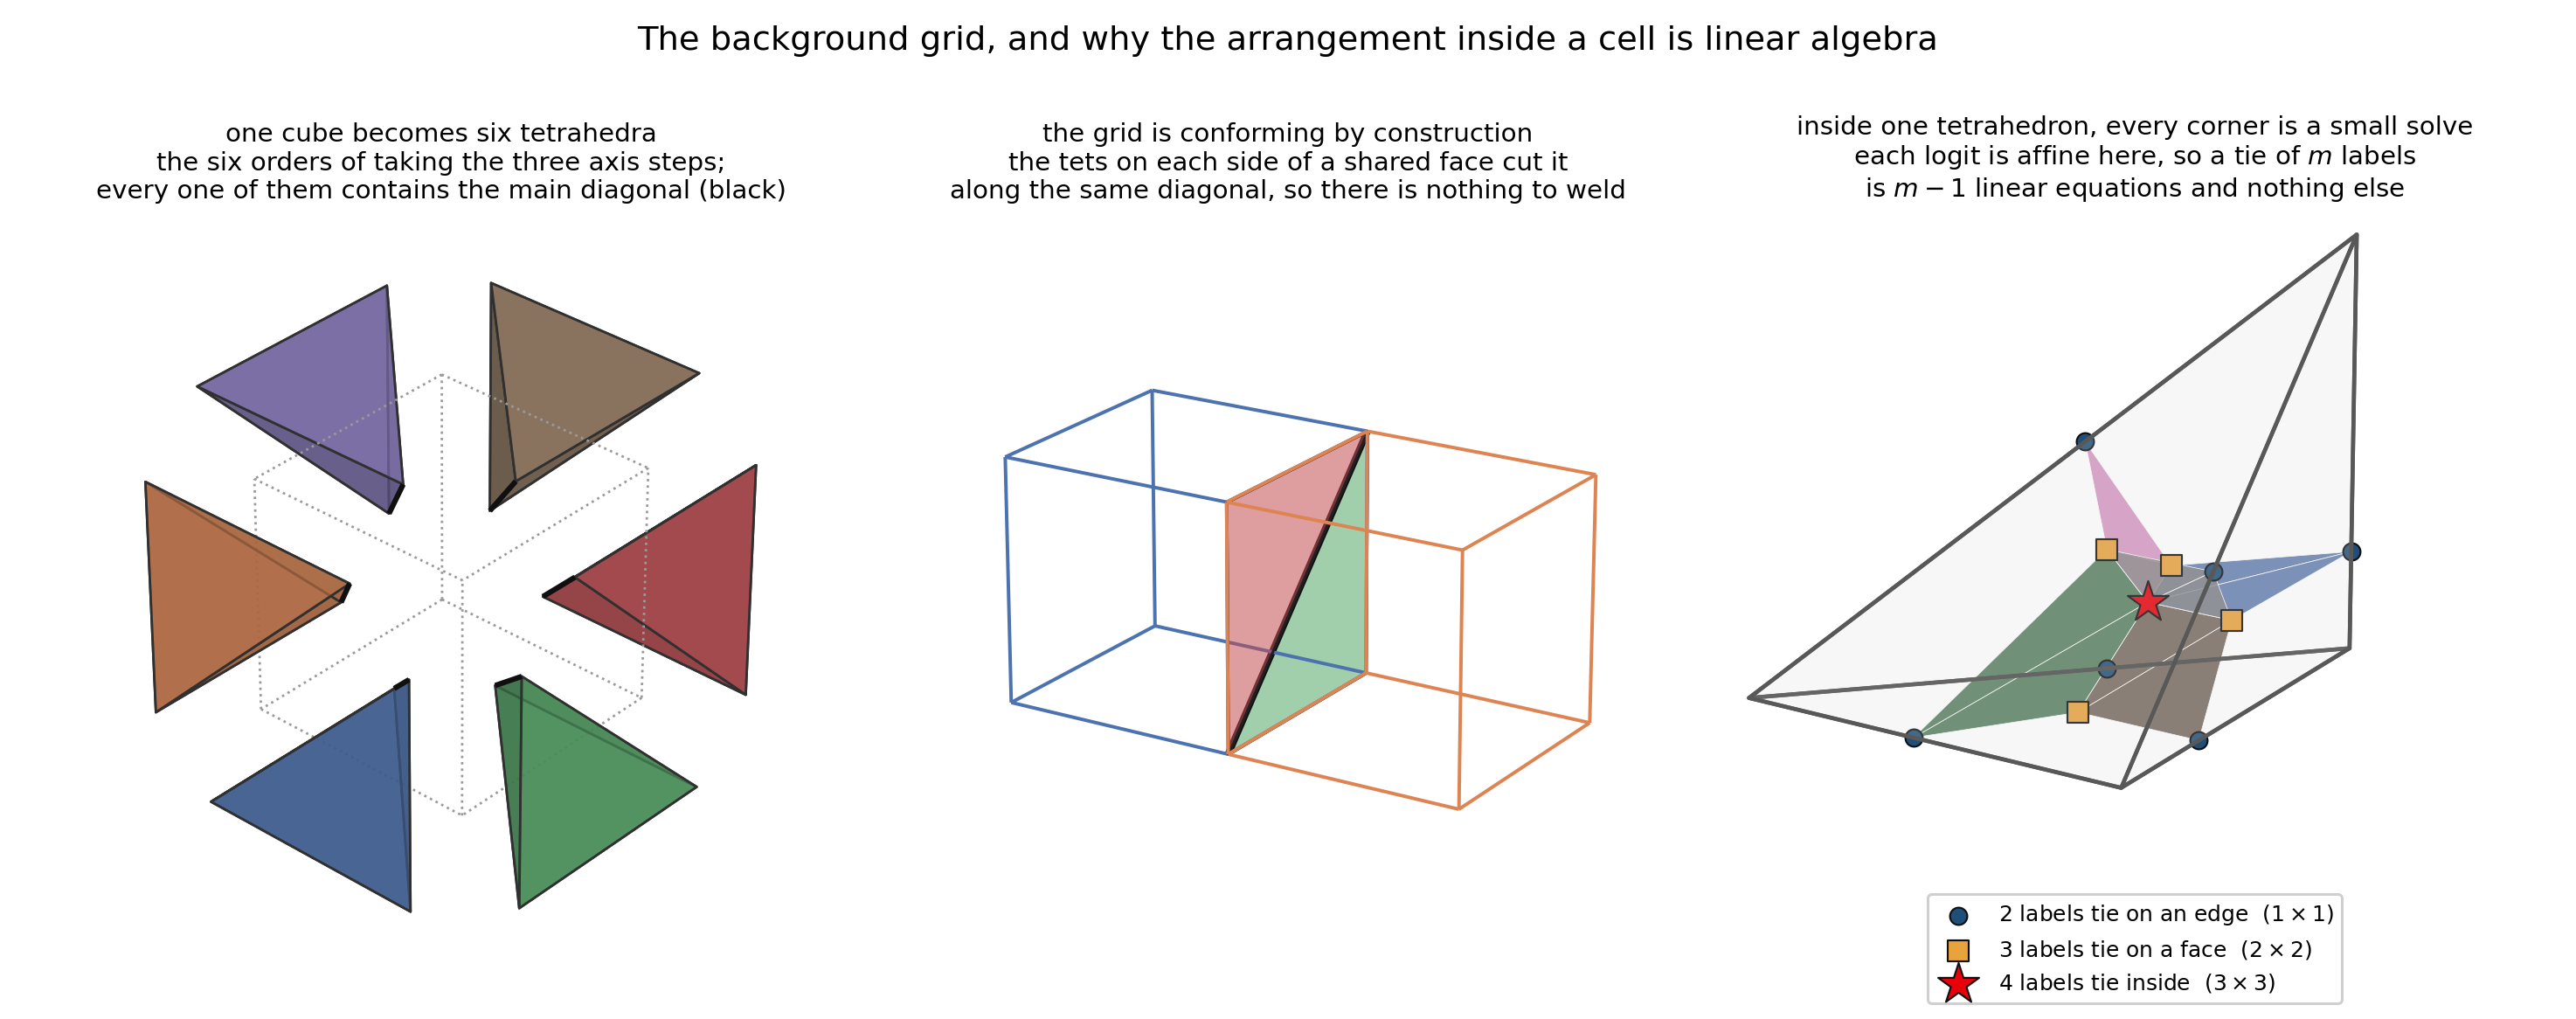
\includegraphics[width=0.88\linewidth]{tetrahedra.png}
\caption{The background grid and the solves it induces. Left: one cube cut into
six tetrahedra, drawn exploded and viewed almost along the main diagonal that
all six share. Centre: two neighbouring cubes induce the same diagonal on their
shared face, which is why the grid is conforming without a welding step. Right:
inside one tetrahedron every logit is affine, so a tie of $m$ labels is $m-1$
linear equations --- here six two-label ties on edges, four three-label ties on
faces and one four-label tie in the interior, which is the whole vertex set of
the arrangement in that cell.}
\label{fig:tetrahedra}
\end{figure*}

\section{Why per-cell case analysis fails in 3D}
\label{sec:failure}

The standard way to extract an isosurface is to classify each cell by the
labels at its corners and look up the resulting patch structure in a
table~\cite{lorensen1987, doi1991}. Extended to $K$ labels on tetrahedra, the natural
table is dictated by a counting argument: place one crossing on each edge whose
two endpoints differ, one triple point inside each face showing three distinct
corner labels, and one quadruple point inside each tetrahedron showing four.

We implemented this first. It is wrong, and instructively so.

\paragraph{The assumption.} A face with corner labels $\{k,l,m\}$ is assumed to
contain the point where $\interp_k = \interp_l = \interp_m$. That point exists
--- three affine functions on a plane generically tie somewhere --- but nothing
forces it to lie \emph{inside the face}. It can lie outside, in which case the
three regions still all appear in the face but never meet there: one of them
separates the other two, and the face's argmax partition has no interior vertex
at all. Figure~\ref{fig:multifeature} shows a real instance. The case table then
manufactures a triple point outside the cell that claimed it and builds patches
from it.

\paragraph{Why refinement does not help.} In 2D the analogous assumption is
benign, because the triple set is a discrete point set: a triangle either
contains a triple point or has at most two labels, and the exceptions vanish
under refinement. In 3D the triple set is a \emph{curve}, and the argument is a
self-similarity one. Take a generic point of a triple curve, where the three
normals $g_k - g_l$ are in general position, and rescale the neighbourhood by
$h$: the field tends to its linearisation, so what a cell of size $h$ sees
converges to a fixed cone of three half-planes meeting along a line,
independent of $h$. Both the faces carrying three labels and those whose
equal-logit solve falls outside them are then determined by where that cone
falls relative to the cell, and refinement resamples that placement rather than
sharpening it. The misread fraction therefore tends to a constant fixed by the
cone, and the constant is nonzero because the offending placements occupy an
open set. The number of faces involved is the number of cells meeting a
one-dimensional set, which is $\Theta(h^{-1})$.

\paragraph{Measurement.} Table~\ref{tab:failure} bears this out on a five-site
power diagram. The count of three-label faces grows as $205$, $402$, $608$
across resolutions $16$, $32$, $48$, close to the $\Theta(h^{-1})$ predicted,
while the fraction of them containing no interior triple point moves from
$49.8\%$ to $47.4\%$: non-monotone, and not approaching zero. The right panel
of Figure~\ref{fig:failure} repeats the sweep on a second, unrelated power
diagram, where the rate runs $40.0\%$, $42.1\%$, $43.8\%$, $42.0\%$ over
resolutions $8$ to $48$ --- flat, and if anything rising. Neither field is
evidence that the rate converges; both are consistent with the constant the
argument above predicts, and we claim no more than that. Figure~\ref{fig:failure} shows the geometric
consequence and Table~\ref{tab:exact} the numerical one: on a piecewise-planar
power-diagram cell, which a correct extractor recovers exactly at any
resolution, the corner-label method attains a relative volume error of
$7.3\times10^{-2}$ at resolution $48$ and a convergence rate of $0.47$.

\paragraph{Relation to the classical tables.} This is not a strawman --- a
corner-indexed table is what the multi-material lineage surveyed above is built
on, and what CGAL indexes today~\cite{hege1997, cgalmesh3} --- but it is worth
saying why those methods survive the objection and a neural field does not.
With integer labels at the nodes the eight corner labels \emph{are} the data,
so a table indexed by them loses nothing: there is no finer truth to be wrong
about, only a reconstruction convention, which Hege et al.~\cite{hege1997} fix
by $6^3$ subsampling and report as topologically correct, which for integer
probabilities it is. The moment the node values are real numbers --- a
segmentation network's logits, a power diagram, any field one intends to
optimise --- the corner labels stop determining the partition, recording which
label wins at eight points and saying nothing about where the ties lie. The
table then answers a question the data no longer poses, and
Table~\ref{tab:failure} is the size of the discrepancy.

\paragraph{This is not the ambiguity the decider resolves.} The known repair
for case tables, the asymptotic decider~\cite{nielson1991} and the
topologically complete variants following it, does not apply. Those methods
resolve \emph{ambiguity}: several topologies fit the same corner labels, one
must be chosen, and the choice is made by going back to the interpolated values
precisely because the labels alone do not determine the answer. That diagnosis
is ours, one label short. The corner labels of a three-label face are not
ambiguous; the table's error is to assert that the three regions meet inside
the face when the equal-logit solve places their meeting point outside it, and
no predicate on the eight corners can detect that, because the location of the
tie is not a function of the labels. The decider's own logic carried to $K$
labels is to stop reading labels and solve for the tie, which is what
Section~\ref{sec:method} does.

A second, independent shortfall of the same table is that it allows only one
feature per cell, where an edge can carry two crossings
(Figure~\ref{fig:multifeature}, left) and a face two triple points. Across five
test fields at one resolution we count $205$ multi-crossing edges and $8$
multi-triple-point faces (supplementary material). Dual
contouring~\cite{ju2002} and its multi-material extension~\cite{mmdc2023}
remove the table but keep the budget: one vertex per cell cannot carry two
triple points on one face, and the minimiser of a least-squares functional is
not a solution of the equal-logit equations even on affine logits, where an
exact solution exists and we return it.

\begin{table}[tbp]
\centering
\caption{Failure rate of corner-label case analysis on the five-site power
diagram of Table~\ref{tab:exact}. A three-label face whose triple point lies
outside it is one the case table misreads. The rate is non-monotone and does
not approach zero; the right panel of Figure~\ref{fig:failure} shows the same
for a second field.}
\label{tab:failure}
\begin{tabular}{@{}rrrr@{}}
\toprule
resolution & three-label faces & misread & rate \\
\midrule
16 & 205 & 102 & 49.8\% \\
32 & 402 & 169 & 42.0\% \\
48 & 608 & 288 & 47.4\% \\
\bottomrule
\end{tabular}
\end{table}

\begin{figure*}[tbp]
\centering
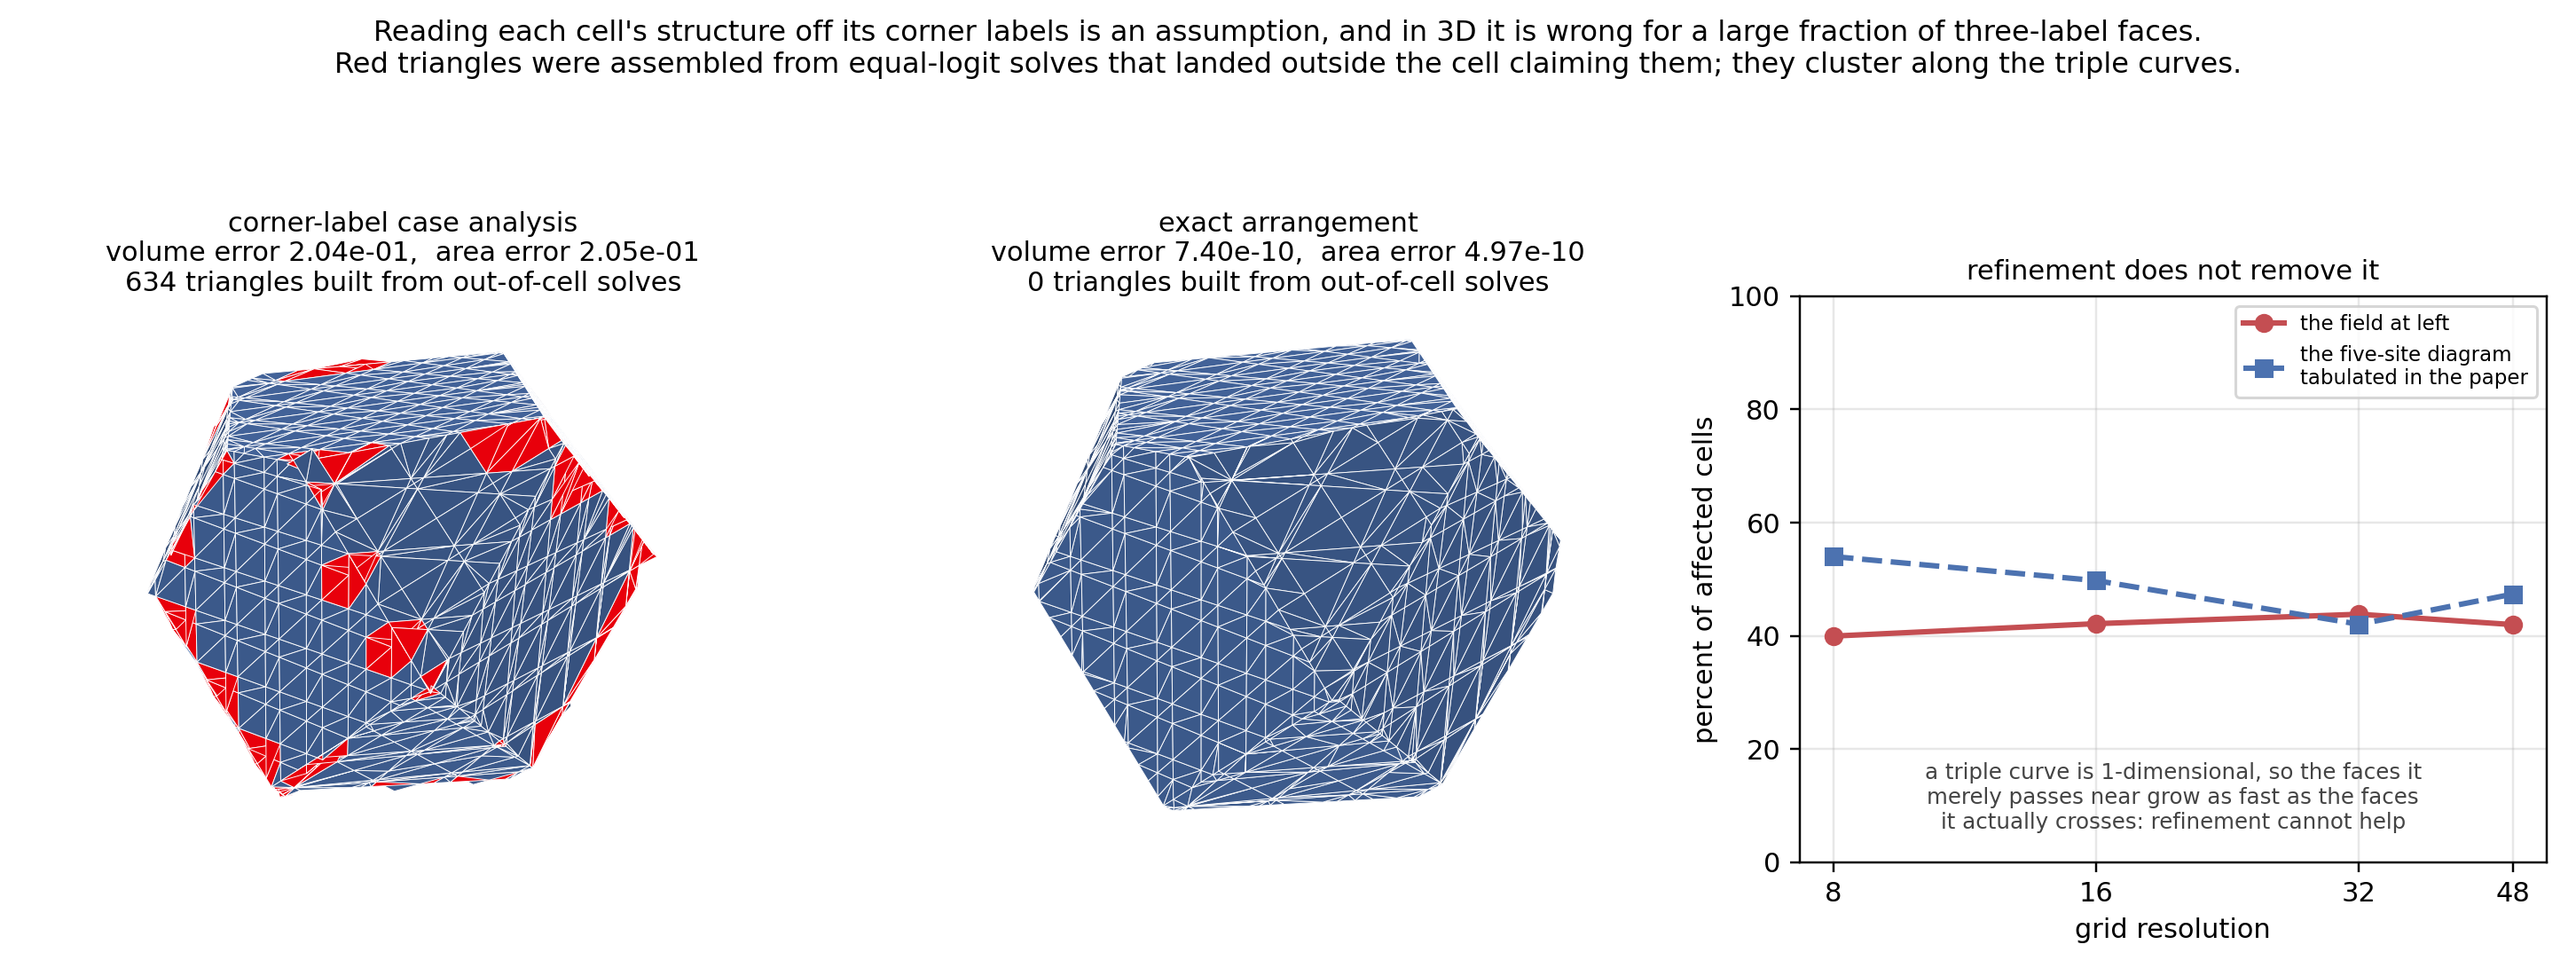
\includegraphics[width=0.88\linewidth]{corner_label_failure.png}
\caption{The corner-label failure, shown three ways. Left and middle: the same
region of the same field at the same resolution, extracted
two ways. Red triangles were assembled from equal-logit solves that landed
outside the cell claiming them; they concentrate along the triple curves, where
the corner-label reading has to guess. Left: $634$ such triangles and $20\%$
volume error, at resolution $16$. Middle: none, and $7.4\times10^{-10}$. Right:
the misread rate against resolution, for this field and for the five-site
diagram of Table~\ref{tab:failure}. Neither approaches zero.}
\label{fig:failure}
\end{figure*}

\section{Method}
\label{sec:method}

We extract \eqref{eq:dregion} exactly. There are two routes to it, and the
choice between them is the whole of our departure from Du et
al.~\cite{du2022}, so it belongs before the construction rather than after.
Theirs is incremental: within each tetrahedron they maintain a cell complex,
insert one function at a time, split the elements its level set crosses and
merge the ones it dominates, never forming a vertex coordinate at all
(Section~\ref{sec:related}). Ours is direct: enumerate candidate label sets,
solve each tie in closed form, and keep the solutions that pass an explicit
containment and dominance test.

Of the two, theirs is the more sophisticated algorithm and by some distance the
more robust one. Ours buys the explicit, differentiable vertex, and with it a
second property: the work per entity is uniform enough that the whole grid is
processed in a fixed number of batched array operations rather than
tetrahedron by tetrahedron. Read the construction below as the simplest thing
with those two properties, not as an improvement on the arrangement algorithm
it stands beside.

Three facts make the direct route cheap. Algorithm~\ref{alg:extract} is the
whole of it; the subsections below justify each step.

\begin{algorithm}[tbp]
\caption{Exact arrangement of the $P_1$ interpolant of the logits. Every loop
ranges over independent entities and runs as a batched array operation. No step
consults a case table; the two inexact comparisons, simplex containment and
dominance, are discussed in Section~\ref{sec:predicates}.}
\label{alg:extract}
\begin{algorithmic}[1]
\Require field $f:\Omega\to\R^K$, resolution $n$, perturbation $\varepsilon$
\Ensure triangles tagged by ordered label pair; triple-curve segments
\State build a conforming tetrahedral grid: nodes $V$, tetrahedra $T$
\State $L \gets f(V)$, displaced by $\varepsilon$
  \Comment{Section~\ref{sec:degeneracy}}
\State $\lab(v) \gets \arg\max_k L_v[k]$
\ForAll{edges $(a,b)$ with $\lab(a) \neq \lab(b)$, label pairs $\{k,l\}$}
  \State $t \gets g_a/(g_a - g_b)$, \; $g = L[k] - L[l]$
  \If{$t \in (0,1)$ and no label beats $k$ there}
    \State emit crossing
  \EndIf
\EndFor
\For{$m = 3, 4$}
  \Comment{triple points on faces, then quadruple points}
  \State seed each cell's label set from its boundary entities
  \Repeat
    \ForAll{cells and label sets $S$, $|S| = m$}
      \State solve $A(L)\,\lambda' = b(L)$
        \Comment{$(m{-}1) \times (m{-}1)$, \eqref{eq:solve}}
      \If{$\lambda'$ in the simplex and no label beats $S$}
        \State emit vertex
      \ElsIf{$\lambda'$ in the simplex but label $k$ beats $S$}
        \State add $k$ to the cell's label set
      \EndIf
    \EndFor
  \Until{no label set grew}
\EndFor
\ForAll{groups of incidences by (tetrahedron, label pair)}
  \State sort the corners about the normal and fan
    \Comment{Proposition~\ref{prop:convex}}
\EndFor
\State pair same-triple vertices within each tetrahedron into segments
\end{algorithmic}
\end{algorithm}

\subsection{Regions are convex inside each cell}

On a tetrahedron $\tet$, $\dregion{k} \cap \tet$ is the intersection of $\tet$
with the half-spaces $\{\interp^\tet_k \ge \interp^\tet_j\}$, each bounded by a
plane because $\interp^\tet_k - \interp^\tet_j$ is affine. So
$\dregion{k}\cap\tet$ is a convex polytope and each interface patch
$\dregion{k}\cap\dregion{l}\cap\tet$ is a convex polygon. A convex polygon is
determined by its corner set: sorting the corners by angle about the patch
normal and fanning yields a correct, consistently oriented triangulation. There
is no case analysis to get wrong, and --- unlike a table-driven fan --- it
cannot fold.

\subsection{Every corner is a small linear solve}
\label{sec:solve}

A corner of a patch is a $0$-dimensional face of the polyhedral complex, so it
is cut out by three independent active constraints drawn from the four face
planes of $\tet$ and the bisector planes $\{\interp_k = \interp_j\}$. If $m$
labels tie at the point, the bisectors contribute $m-1$ independent constraints
and the tetrahedron's own faces contribute the remaining $3-(m-1)$, placing the
point on a face of $\tet$ of dimension $m-1$. This yields exactly three kinds of
vertex, and bounds $m$ by $4$:
\[
\begin{array}{lll}
  \text{on a grid edge} & \interp_k = \interp_l & \text{crossing} \\
  \text{on a grid face} & \interp_k = \interp_l = \interp_m & \text{triple point} \\
  \text{inside a tetrahedron} & \interp_k = \interp_l = \interp_m = \interp_p
    & \text{quadruple point.}
\end{array}
\]
Crucially the key is the \emph{label set}, not the cell. An edge may carry
several crossings and a face several triple points, which is precisely what the
case analysis could not express.

Each is a closed-form solve. Write the tied set as $S = \{l_0,\dots,l_{m-1}\}$.
The point lies on the $(m-1)$-dimensional face of $\tet$ whose corner logits are
$L_0,\dots,L_{m-1}$, on which the interpolated logit of label $k$ is
$\sum_a \lambda_a L_a[k]$. Each equality $\interp_{l_0} = \interp_{l_r}$, for
$r = 1,\dots,m-1$, is therefore affine in the free barycentric coordinates
$\lambda' = (\lambda_1,\dots,\lambda_{m-1})$, the remaining one being
$\lambda_0 = 1 - \sum_{a \ge 1} \lambda_a$. Collecting them gives an
$(m-1) \times (m-1)$ system
\begin{align}
  A(L)\,\lambda' &= b(L), \label{eq:solve} \\
  A_{r a} &= \big(L_a[l_0] - L_a[l_r]\big)
             - \big(L_0[l_0] - L_0[l_r]\big), \nonumber \\
  b_r &= -\big(L_0[l_0]-L_0[l_r]\big), \nonumber
\end{align}
with $A$ and $b$ linear in the node logits. For a crossing $m=2$,
\eqref{eq:solve} is scalar and reduces to the familiar ratio
$t = g_0/(g_0-g_1)$ with $g$ the logit difference at each endpoint; triple and
quadruple points give $2\times2$ and $3\times3$ systems.

A tie exists for any label set; it is a vertex of the arrangement only if it
lies in its simplex \emph{and} no other label beats it there. We test both, over
all $K$ labels rather than only those the cell's boundary suggested, so that two
cells sharing a face cannot disagree about whether their common point is real.

\subsection{Which label sets to try}

Enumerating all $\binom{K}{m}$ label sets per cell is wasteful, so candidates
are seeded from the labels reachable on the cell's boundary. That seed can miss
a label occupying a cell's interior without touching its edges, and missing one
is not harmless: the tie it should have produced is a corner of a neighbouring
patch, so omitting it punches a hole.

We therefore refine the seed rather than trust it. Whenever a tie lands inside a
cell but is beaten, whatever beat it is by definition the argmax somewhere in
that cell, hence present in it; that label joins the cell's set and the
enumeration repeats. The loop is run to a fixed point rather than for a fixed
number of passes, and terminates because the label sets only grow and it stops
on the first round that fails to grow them, bounding it by $K$ passes; across
the power-diagram and neural fields at resolutions $16$ to $48$ it never needed
more than two. This self-correction is
what takes the power-diagram results in Table~\ref{tab:exact} from nearly exact
to exact.

Refinement recovers a missing label only when some enumerated tie lands inside
the cell and is beaten by it. A region small enough to lie strictly inside one
tetrahedron leaves no such evidence; that is the one residue, and
Section~\ref{sec:limitations} describes both it and the screen we run for it.

The incremental route has to answer the same question and answers it the other
way. Du et al.~\cite{du2022} treat a function as active in a tetrahedron unless
some other function exceeds it at all four vertices --- a criterion they note
admits functions that turn out not to contribute, and whose surplus they accept
for its simplicity. Their error is over-inclusion, which costs time. Ours is
omission, which would cost a hole, so it has to be repaired rather than
tolerated. What makes the repair available is that a beaten tie carries the
evidence of what is missing: the label that beat it is the argmax at a point of
the cell, hence present in it, so the enumeration converges by being told
precisely what it failed to guess.

\subsection{Assembly}
\label{sec:assembly}

Every vertex is incident to the interfaces of all pairs drawn from its tied
label set: a crossing contributes to one pair, a triple point to all three of
its pairs, a quadruple point to all six. Grouping these incidences by
(tetrahedron, label pair) gives each patch its corner set, which is then fanned
as described above. Triple-curve segments are recovered as the pairs of
same-triple vertices within a tetrahedron.

\subsection{Cost}
\label{sec:cost}

Each candidate label set costs one solve of size at most $3\times3$ and one dominance test
against all $K$ labels, so a tetrahedron whose candidate set holds $L$ labels
costs $O(\binom{L}{4}K)$ at the quadruple level and correspondingly less below
it. The incremental construction it replaces costs $O(L^3)$ on the same
tetrahedron~\cite{du2022}. The direct route is therefore asymptotically the
worse of the two, and is chosen anyway.

What makes that affordable is that $L$ is not $K$ and does not grow with it.
Across the five test fields of Section~\ref{sec:experiments} at resolution
$24$, each with $82\,944$ tetrahedra, the mean candidate set holds between
$1.10$ and $1.26$ labels and no tetrahedron in any of them holds more than
four --- including the $K=6$ neural field.
The binomial never opens up, and what remains is a fixed, uniform quantity of
work per entity, which is exactly the property that lets every edge, face and
tetrahedron be processed in a handful of batched array operations and the
reverse sweep be an ordinary autograd pass.

Measured, the cost behaves as that description predicts. Refining a $K=6$ power
diagram from $24\,576$ to $3\,072\,000$ tetrahedra, a factor of $125$, takes
wall time from $0.08$ to $11.0$\,s --- linear in the tetrahedron count, with
the cost per tetrahedron flat between $3.1$ and $3.6\,\mu$s across the whole
range. Raising $K$ from $3$ to $16$ at fixed resolution costs a factor of
$2.7$, not a binomial, and the mean candidate set grows only from $1.06$ to
$1.18$ labels. What does bound the method is memory rather than time: peak
working set runs at roughly half a kilobyte per tetrahedron, $1.4$\,GB at three
million, and that is what limits the resolution reachable on one machine. The
sweep is tabulated in the supplementary material. On an input that did
concentrate many labels into single cells the balance would reverse, and the
incremental construction would be the better algorithm.

\subsection{Gradients}

Positions come from \eqref{eq:solve}, which is a linear solve in the node
logits, so reverse-mode automatic differentiation through
$L = f_\theta(\text{nodes})$ gives exact gradients. Two design points make this
work in practice. First, all \emph{combinatorial} decisions --- which label sets
tie, whether a tie is inside its simplex, which label wins --- are taken on a
detached copy of the logits, while positions are computed with the graph intact;
the discrete structure is therefore decided without gradients and the geometry
carries them. Second, no iteration is involved. An earlier version of this work
located vertices by bisection and Newton iteration and reattached gradients
through the implicit function theorem, because a root found by iteration has no
usable autograd path. Extracting the arrangement of the interpolant removes the
need: the interpolant is affine on each cell, so the root is a linear solve
rather than a limit.

\subsection{Degeneracy}
\label{sec:degeneracy}

The construction reads the arrangement off strict inequalities, so exact
coincidences are the one thing that can break it, and on a regular grid they are
not rare. Two occur immediately. A node can lie exactly on an interface, which
happens for every sphere whose radius the grid step divides; the crossing on each
incident edge then sits at the node, is rejected as out of range, and leaves a
hole. A triple curve can meet a grid edge exactly, which happens whenever the
geometry is aligned to round numbers; the three pairwise crossings then coincide
with each other and with a triple point on every incident face, and the patches
around that point are assembled from several copies of one corner.

We resolve both by symbolic perturbation~\cite{edelsbrunner1990}: displace the
node logits by a deterministic amount $\varepsilon$ depending only on the node
and the label. Two properties make this sound. The displacement is shared by
every cell touching a node, so cells still agree on their common boundary and
conformity is untouched; and it is a constant with respect to $\theta$, so
gradients are unchanged. The cost is a position error of $O(\varepsilon)$; at
$\varepsilon = 10^{-9}$ this is ten orders of magnitude below the discretisation
error it sits inside, and Table~\ref{tab:exact} reports it separately so that
the method and its perturbation can be told apart.
Section~\ref{sec:further} measures what it costs as a configuration is driven
towards an actual degeneracy, where the error stays $O(\varepsilon)$ instead of
being amplified by the ill-conditioning.

\subsection{Predicates and tolerances}
\label{sec:predicates}

Three decisions in Algorithm~\ref{alg:extract} are inexact comparisons rather
than exact predicates, and it is worth being precise about them, since exact
predicates are what the construction we compare against uses instead. All
three carry the same slack $\tau = 10^{-12}$. A crossing on an edge is kept
only if its parameter satisfies $\tau < t < 1 - \tau$; a solved tie is kept
only if it lies in its simplex, $\lambda_a \ge -\tau$; and a label counts as
beating the tied set only if it exceeds it by more than $\tau$. The first two
point opposite ways --- one discards a marginal case, the other admits one ---
because a crossing at a node is already carried by the entities meeting there,
whereas a tie just outside its simplex is carried by nothing else. Two further
constants appear but decide nothing structural: a $10^{-30}$ floor guards the
denominators of the crossing and tie solves against division by zero, and a
$10^{-9}$ window marks which vertices lie on the domain boundary, which the
closure check uses to excuse sides that have no partner by construction.

Neither the slack nor the perturbation endangers conformity. Edges and faces are deduplicated into global
entities keyed by their sorted node indices before anything is solved, so a
face's triple point is computed once, from that face's three corner logits in a
canonical order, and dominance is evaluated at the resulting point over all $K$
labels. The two tetrahedra sharing the face read one verdict rather than
agreeing on two; Proposition~\ref{prop:conform} is a statement about that
shared computation, not about the slack in it. Nor does $\tau$ compete with
the perturbation, though the two are not measured in the same units: $\tau$ is
a slack on barycentric coordinates and dominance margins, while the
perturbation displaces the logits upstream of both, each by
$\mathrm{frac}\cdot\varepsilon\cdot\max_j |L_j|$ with
$\mathrm{frac} \in (-\tfrac12, \tfrac12)$. At $\varepsilon = 10^{-9}$ that
displacement is typically several orders of magnitude above $\tau$, so a
configuration close enough for $\tau$ to decide it is one the perturbation has
usually already moved away from. The implementation counts patches left with fewer than three corners,
which is how a corner rejected by $\tau$ announces itself, and that count is
zero on every field reported here.

\begin{figure*}[tbp]
\centering
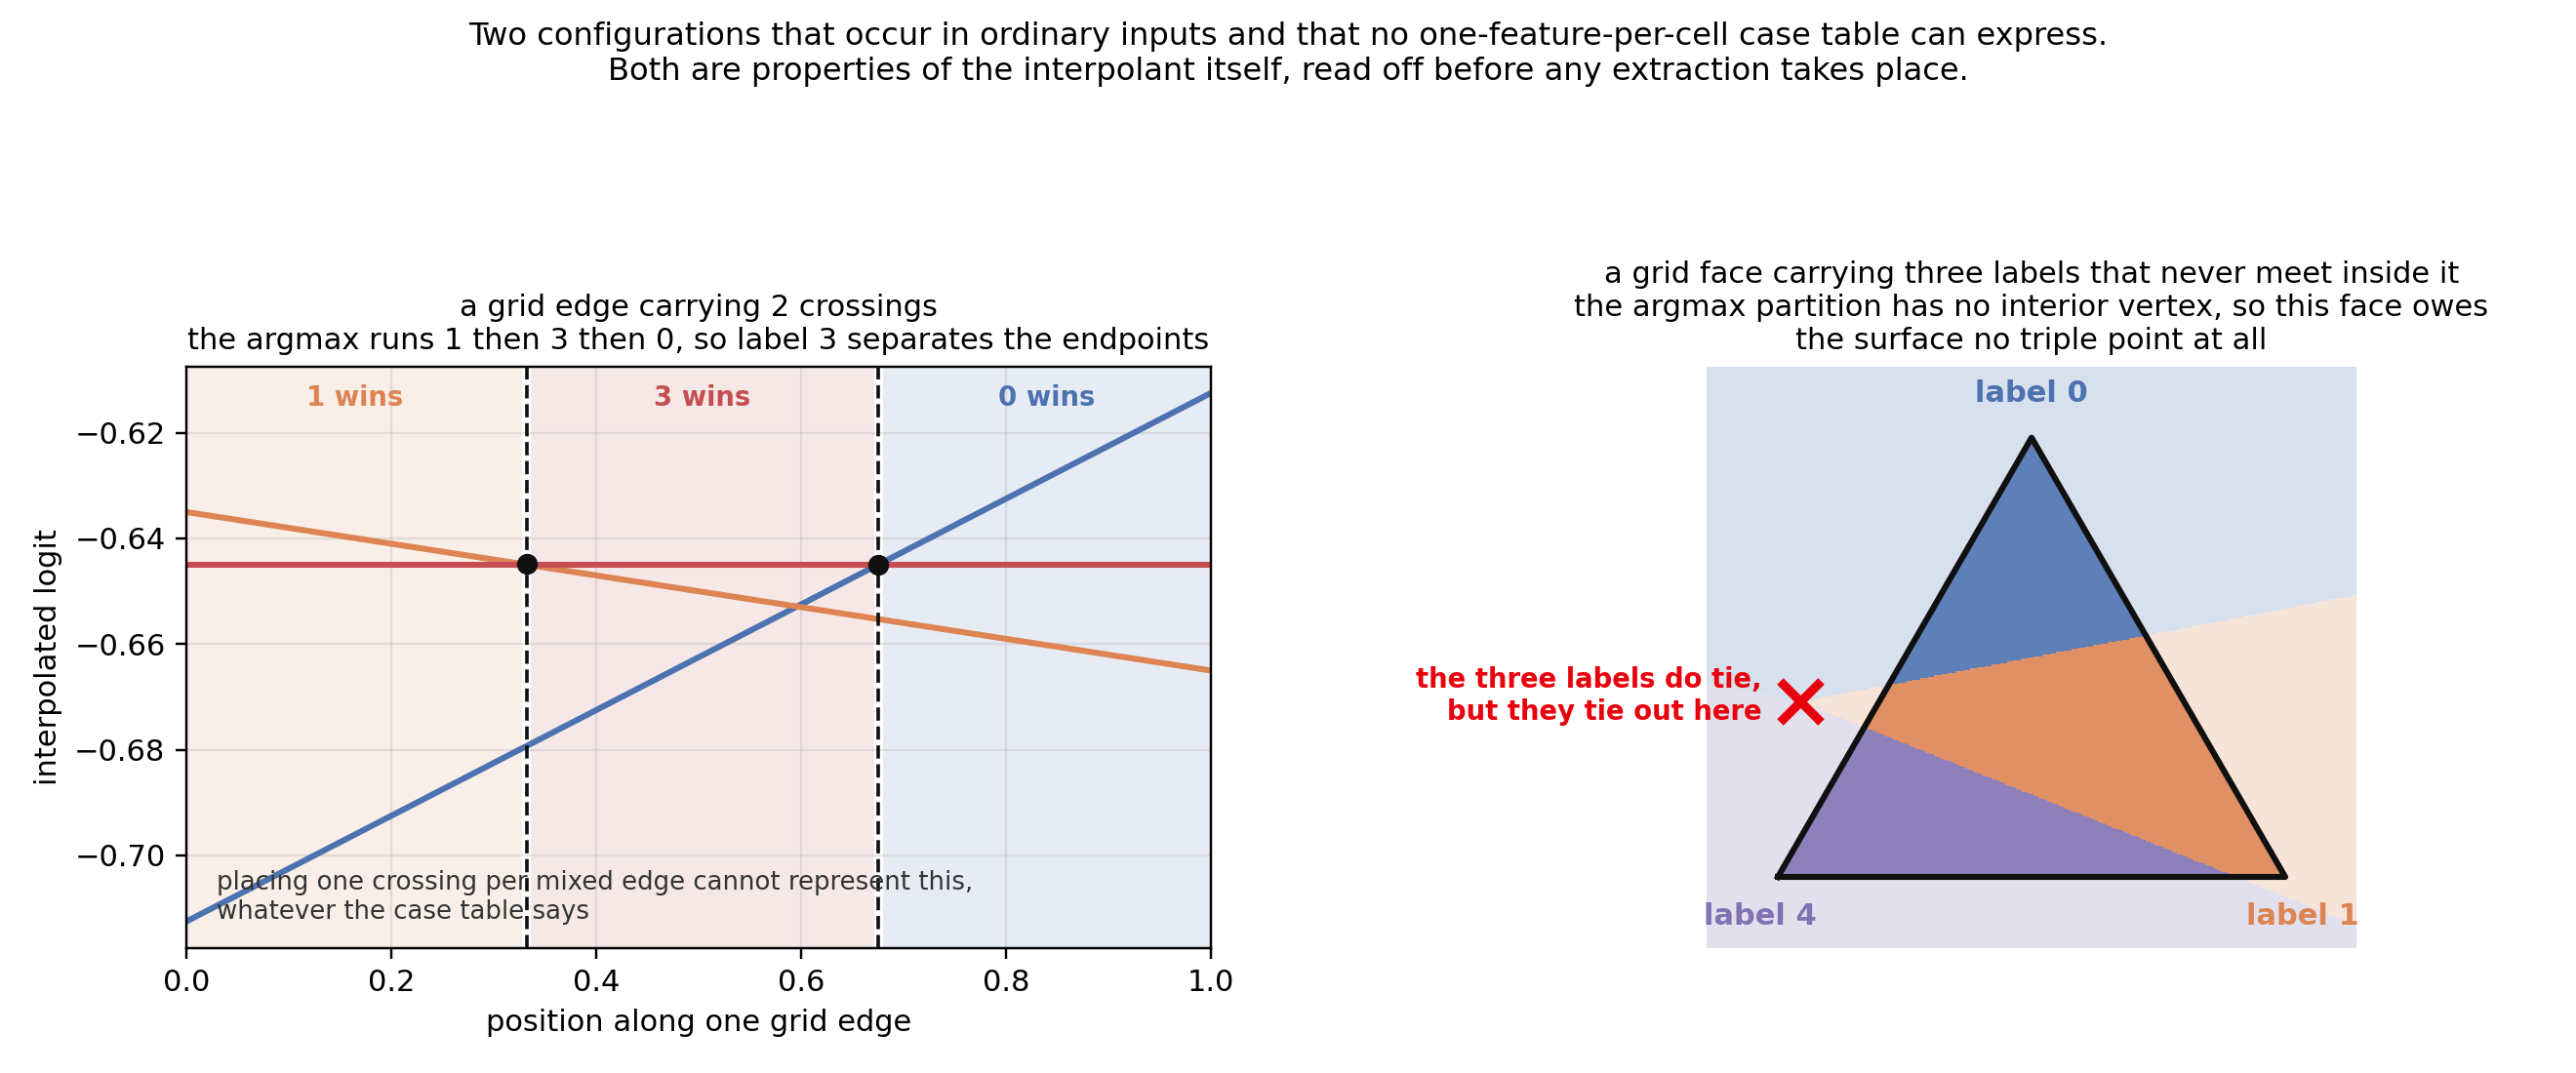
\includegraphics[width=0.88\linewidth]{multi_feature_cells.png}
\caption{Two configurations that occur in ordinary inputs and that no
one-feature-per-cell table can express. Left: a grid edge on which the argmax
changes twice, so a single crossing cannot describe it. Right: a grid face
carrying three labels whose regions never meet inside it --- the three labels do
tie, but outside the face, so the face owes the surface no triple point. Both
panels are read off the interpolant, before any extraction.}
\label{fig:multifeature}
\end{figure*}

\section{Guarantees}
\label{sec:guarantees}

\noindent What follows are properties the construction has, not tolerances it
meets: each is a consequence of the interpolant being affine within a cell.
They are stated for exact arithmetic and for a \emph{generic} field --- one in
which no tie is degenerate, no label is exactly equal to a tied set, and no
vertex lands exactly on the boundary of its simplex. That genericity is not an
idealisation introduced to make the proofs work: it is the condition the
symbolic perturbation of Section~\ref{sec:degeneracy} exists to establish, and
Propositions~\ref{prop:classify} and~\ref{prop:diff} are false without it. All
six proofs are short and are given in the supplementary material.

\begin{proposition}[Convexity]
\label{prop:convex}
For every tetrahedron $\tet$ and every $k$, $\dregion{k}\cap\tet$ is a convex
polytope, and for every pair $k \neq l$ the patch
$\dregion{k}\cap\dregion{l}\cap\tet$ is a convex polygon.
\end{proposition}

\begin{corollary}
A patch is the convex hull of its corners. If it is two-dimensional and its
corners are distinct, sorting them by angle about the patch normal and fanning
produces a triangulation whose triangles are non-degenerate, consistently
wound, and non-overlapping. A patch that is not two-dimensional, or whose
corners are not distinct, would emit fewer
than three corners, which the implementation counts (Section~\ref{sec:predicates}).
\end{corollary}

\begin{proposition}[Conformity]
\label{prop:conform}
Let $\varphi$ be a face shared by $\tet$ and $\tet'$. The vertices the method
places on $\varphi$ are the same vertices for $\tet$ and for $\tet'$, as
floating-point values and as indices.
\end{proposition}

\noindent This is why no welding, snapping or tolerance-based merging appears
anywhere in the method: where two cells both place a vertex on their shared
face, it is the same vertex, not two within a tolerance of each other. Closure
needs the further fact that neither cell \emph{omits} a corner, which the
proposition does not supply and which we therefore check rather than claim:
across forty randomly drawn fields, seeded disjointly from every field used
elsewhere in the paper, every triangle side is used exactly twice with opposite
winding except on triple curves and at the domain boundary.

\begin{proposition}[Exactness on affine logits]
\label{prop:affine}
If every $f_k$ is affine then $\interp = f$ on $\Omega$, and the extracted
complex is the exact argmax partition of $f$ for any background grid on which
every non-empty region meets some cell boundary. In particular power diagrams,
and hence Voronoi diagrams, are recovered exactly at any resolution, in the
sense that the only error is the rounding of the solves.
\end{proposition}

\begin{proposition}[Vertex classification]
\label{prop:classify}
At most four labels tie at any vertex of the extracted complex, and a vertex at
which $m$ labels tie lies on a face of its tetrahedron of dimension $m-1$.
\end{proposition}

\begin{proposition}[Plateau's condition holds identically]
\label{prop:plateau}
Let three patches meet along a triple curve of labels $\{k,l,m\}$ inside a
tetrahedron, and let $g_k = \nabla \interp^\tet_k$ be the (constant) gradients.
The three patch normals $n_{kl} = g_k - g_l$, $n_{lm} = g_l - g_m$,
$n_{mk} = g_m - g_k$ are orthogonal to the curve and satisfy
\[
  n_{kl} + n_{lm} + n_{mk} = 0 .
\]
Consequently the three dihedral angles are $120^\circ$ exactly if and only if
$\|n_{kl}\| = \|n_{lm}\| = \|n_{mk}\|$.
\end{proposition}

\begin{remark}
The vanishing sum is the Herring force-balance condition at a triple junction
with unit surface tensions~\cite{herring1951, taylor1976}, so the extractor
does not approximate Plateau's law and converge to it but satisfies the
balance identically, the $120^\circ$ angles appearing whenever the field itself
is balanced. The price of an identity holding by construction is that
verifying it on the normals cannot fail; what can fail, and is measured in
Section~\ref{sec:doublebubble}, is the angle between the triangles actually
emitted on a curved interface.
\end{remark}

\begin{proposition}[Differentiability]
\label{prop:diff}
Fix $\theta_0$ at which $\theta \mapsto f_\theta$ is differentiable and every
predicate deciding the structure holds strictly: no tie is degenerate
($\det A \neq 0$ in \eqref{eq:solve} for every emitted vertex), no vertex lies
on the boundary of its simplex, every non-tied label is strictly beaten, and
every node's argmax margin is strictly positive. Then the combinatorial
structure is constant in a neighbourhood of $\theta_0$, every vertex position
is a differentiable function of $\theta$ there, and reverse-mode automatic
differentiation realises its exact Jacobian.
\end{proposition}

\noindent The excluded set is where the topology of the output changes --- a
vertex entering or leaving a cell, or a tie becoming degenerate --- which is a
measure-zero set of parameters and is precisely where no extractor can be
differentiable.

\section{Experiments}
\label{sec:experiments}

Multi-material extraction is hard to validate against a mesh produced by another
mesher, so we validate against closed form throughout, and separately against
the one implementation that targets the same partition
(Section~\ref{sec:headtohead}). Three families of test field admit exact
answers:

\begin{description}
\item[Power diagrams.] Affine logits, so by Proposition~\ref{prop:affine} the
correct output is the exact power diagram, independent of resolution. We compute
each cell's volume, per-neighbour facet areas and corner positions analytically
by intersecting half-space triples and testing feasibility, giving ground truth
to machine precision.
\item[Spherical shells.] Concentric regions with exact radii, giving known
interface areas and a curved geometry on which exactness is impossible and the
convergence order is the thing to measure.
\item[Symmetric sector fans.] $K$ regions meeting at a point along the
directions of a regular simplex, so all dihedral angles are known to be
$120^\circ$.
\end{description}

\noindent Neural fields (randomly initialised MLPs on Fourier features, $K=4$
and $K=6$) are included wherever ground truth is not required, to check that
nothing depends on the field being analytic. All arithmetic is float64.
Section~\ref{sec:doublebubble} adds a field with one constant channel, whose
interfaces are spheres meeting a plane, because it contains the standard double
bubble exactly. Section~\ref{sec:2d} reports the 2D instantiation, which we
built first and use for the remaining optimisation studies.

\subsection{Exactness on a power-diagram cell}

Table~\ref{tab:exact} is the central quantitative result. The test cell is a
bounded polytope with $14$ facets and $24$ corners, well inside the domain, with
volume $0.438029035026$ and surface area $3.101575816905$. Because every
interface is planar and every triple curve straight, a correct extractor is
exact at every resolution --- so this table measures correctness, not accuracy.

The arrangement extractor is exact to rounding --- at worst
$2.5\times10^{-16}$ relative, and bit-exact in two of the eight entries --- at
resolution $8$ as much as at $48$. Reported separately is the same extractor with the symbolic
perturbation of Section~\ref{sec:degeneracy} enabled, which costs exactly its
own magnitude and nothing more; Section~\ref{sec:further} measures the same
quantity as the configuration is driven towards an actual degeneracy, where the
cost stays additive rather than amplifying. The corner-label method errs by
$7$--$20\%$ with a fitted convergence rate of $0.47$.

\begin{table*}[tbp]
\centering
\caption{Relative error against an analytically computed power-diagram cell
(volume $0.438029035026$, area $3.101575816905$). Every interface is planar, so
a correct extractor is exact at any resolution. The middle block is exact to
floating-point; the bottom block isolates the cost of the symbolic perturbation
used to resolve degeneracies.}
\label{tab:exact}
\begin{tabular}{@{}lrrrr@{}}
\toprule
& \multicolumn{4}{c}{grid resolution} \\
\cmidrule(l){2-5}
& 8 & 16 & 32 & 48 \\
\midrule
\multicolumn{5}{@{}l}{\emph{corner-label case analysis}} \\
\quad volume & $1.69\!\times\!10^{-1}$ & $2.04\!\times\!10^{-1}$ & $8.73\!\times\!10^{-2}$ & $7.26\!\times\!10^{-2}$ \\
\quad area   & $1.70\!\times\!10^{-1}$ & $2.05\!\times\!10^{-1}$ & $8.48\!\times\!10^{-2}$ & $7.16\!\times\!10^{-2}$ \\
\addlinespace
\multicolumn{5}{@{}l}{\emph{exact arrangement}} \\
\quad volume & $1.3\!\times\!10^{-16}$ & $0$ & $2.5\!\times\!10^{-16}$ & $0$ \\
\quad area   & $1.4\!\times\!10^{-16}$ & $1.4\!\times\!10^{-16}$ & $1.4\!\times\!10^{-16}$ & $1.4\!\times\!10^{-16}$ \\
\addlinespace
\multicolumn{5}{@{}l}{\emph{exact arrangement, perturbed by $10^{-9}$}} \\
\quad volume & $5.4\!\times\!10^{-10}$ & $7.4\!\times\!10^{-10}$ & $2.4\!\times\!10^{-10}$ & $2.3\!\times\!10^{-10}$ \\
\quad area   & $5.7\!\times\!10^{-10}$ & $5.0\!\times\!10^{-10}$ & $2.6\!\times\!10^{-10}$ & $2.9\!\times\!10^{-10}$ \\
\bottomrule
\end{tabular}
\end{table*}

\begin{figure*}[tbp]
\centering
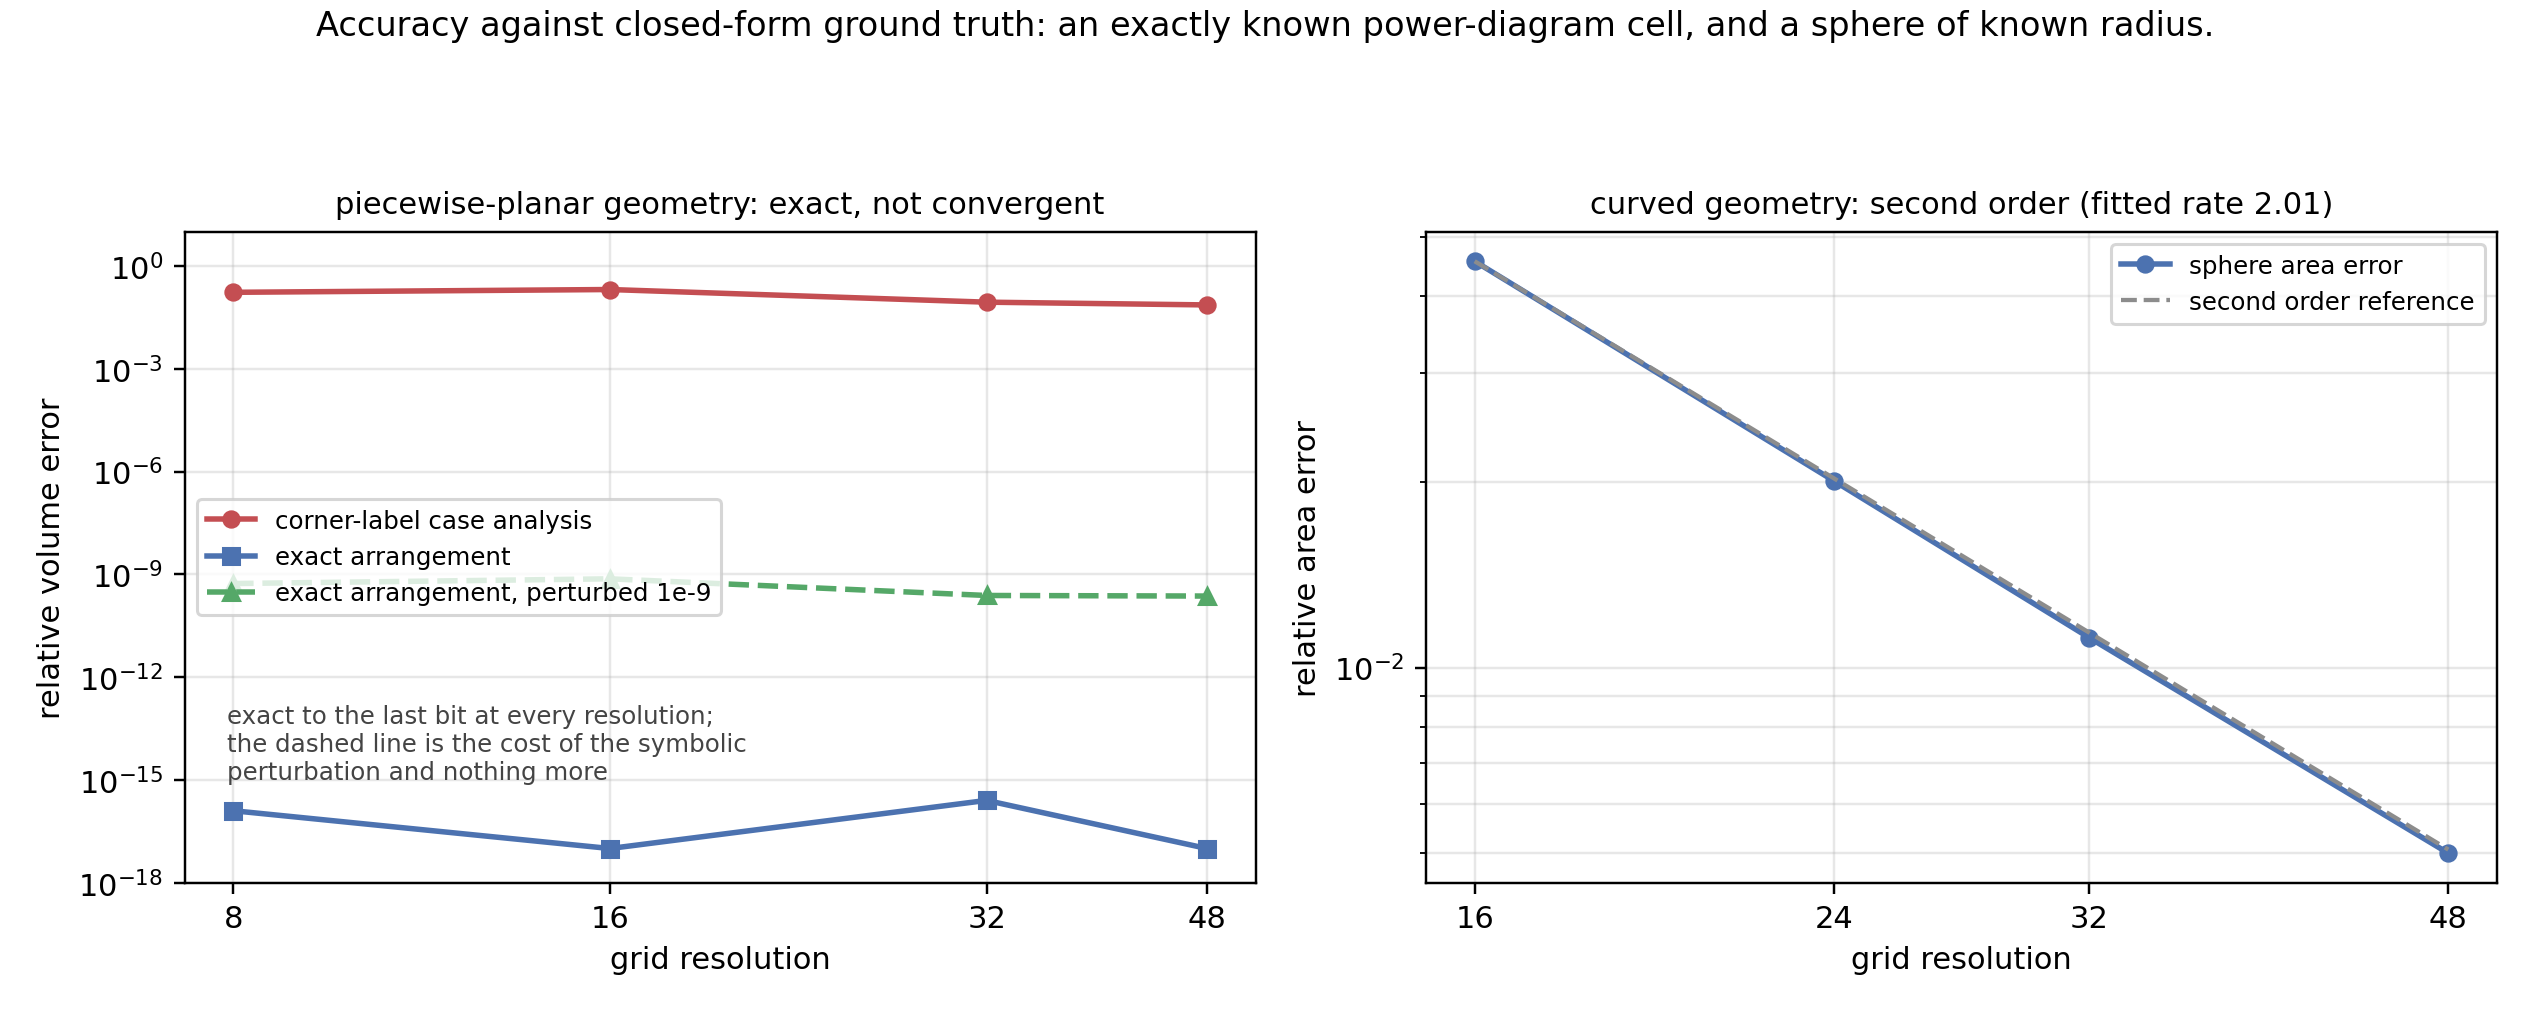
\includegraphics[width=0.88\linewidth]{convergence.png}
\caption{Accuracy against closed form. Left: on piecewise-planar geometry the
arrangement is exact rather than convergent, fourteen orders of magnitude below
the corner-label baseline; the dashed line is the symbolic perturbation. Right:
on a sphere, where exactness is impossible, the area error is second order
(fitted rate $2.01$).}
\label{fig:convergence}
\end{figure*}

\subsection{Agreement with the exact baseline}
\label{sec:headtohead}

Everything above is measured against closed form. The complementary check is
against another implementation of the same object, and the only one we were
able to obtain and run is the public code of Du et al.~\cite{du2022}. The two constructions share no code
and little strategy --- theirs incremental with implicitly encoded vertices,
ours direct with explicit linear solves --- and theirs is correct by
construction, so where the answer is unique, agreement measures ours against
something already known to be right.

Making that mean anything requires removing every difference that is not the
algorithm. Both read the same tetrahedra, passed through their
\texttt{tetMeshFile} input; their loader gains twenty-nine lines so that it can
read per-vertex values for the fields with no closed form, which changes no
line of the arrangement code; and our symbolic perturbation is off, since a
displacement they do not apply would guarantee a mismatch at exactly the
configurations worth comparing. The supplementary material gives the harness in
full, and the container recipe and loader patch are released with our code.

Across eight configurations the two agree on every count --- vertices,
interface polygons, patches, labels, the set of interfaces present --- with
vertex positions coinciding to $10^{-14}$, on up to $663\,552$ tetrahedra of
clinical segmentation output. One of the eight is a control that sends a field
their loader can evaluate analytically down the per-vertex path instead,
testing the addition rather than the extractor. The case list is in the
supplementary material.

The exception is the clinical field as acquired, and it is the exception
Section~\ref{sec:degeneracy} predicts. Ten of its $117\,649$ nodes carry an
exact argmax tie and its smallest nonzero margin is one unit in the last place,
so the arrangement there is genuinely not unique and the two break the tie by
different policies --- theirs symbolic, ours by displacement. The structures
differ by under $0.2\%$ of the vertices, entirely near those coincidences,
while patches, labels and interfaces present still agree; with the perturbation
switched back on, every vertex of theirs lies within $1.7\times10^{-9}$ of one
of ours, and removing the coincidences from the input both extractors read
restores exact agreement. The
concession of Section~\ref{sec:degeneracy} is therefore priced against the
method that does not make it, rather than argued. Cost runs the other way and
we report it plainly: their arrangement takes $16$--$178$\,ms against our
$102$\,ms--$1.2$\,s, our Python against their optimised C++ with a precomputed
lookup table. The ordering is unlikely to reverse, and it is the wrong axis,
since what the exchange buys is a derivative their pipeline does not provide at
any speed.

\subsection{Against a differentiable extractor}
\label{sec:flexicubes}

Section~\ref{sec:related} dismisses the differentiable lineage on the grounds
that its two-manifold guarantee is what a triple curve violates. That is an
argument, and the paper's own claim --- that the construction subsumes the
two-label case --- is a second one. Both are measurable against
FlexiCubes~\cite{shen2023}, and we measure them. Their extractor depends only
on PyTorch, so it runs unmodified; it does run in float32, whereas the rest of
this paper runs in float64, and we note that rather than equalise it, since
float32 is the precision their method is written for, as float64 is ours.

On a fixed field at $K=2$ we are the more accurate. Over a sphere and a torus
at resolutions $16$ to $64$ our relative area error is two to three and a half
times lower, and points drawn uniformly by area from our surface sit closer to
the analytic one by a factor of two to $2.3$ in the root mean square and $1.2$
to $1.7$ at worst; we spend about three times the triangles for it, a primal
mesh on tetrahedra against one dual vertex per cell. Scoring extracted vertices
instead would flatter us, ours being by construction zeros of the interpolant
while a dual vertex is not meant to lie on the surface at all; both measures
are tabulated. The reduction to two labels is real rather than nominal.

Optimisation at $K=2$ is the axis on which they are better. Driving one scalar
grid through both extractors under one Chamfer objective, each tuned over
learning rate and field smoothness, both fit the target point cloud equally
well --- final objectives within $7\%$ --- but their surface lands $0.045$ grid
cells from the analytic ellipsoid in the root mean square against our $0.221$,
and $0.46$ cells at worst against our $3.6$. The mechanism is field noise,
which we report and their averaging damps (Section~\ref{sec:limitations}).
Smoothing the grid buys us the $0.221$ from $0.457$ unsmoothed, at an interior
optimum, so it removes over half our excess without closing the gap while
theirs barely moves either way. On a target additionally requiring a genus
change neither method succeeds, both stalling around two cells.

What the two-label reduction does not survive is a junction. FlexiCubes
consumes one scalar field, so three regions must be asked for one at a time,
each extracted against the union of the others, and the results are then not a
partition: on the standard double bubble they claim $0.90\%$ of the domain
twice and leave $2.9\%$ claimed by none, and refinement only trades one against
the other, taking the total from $3.9\%$ to $3.3\%$ over a threefold
refinement. The decomposition is not what fails, and a control establishes it:
put the same two derived fields to our extractor, one at a time, and the
overlap is zero at every resolution while the labelling error falls from
$0.67\%$ to $0.08\%$. One-vs-rest does yield a partition, provided the
extractor puts its vertices on the zero set it was handed, because the shared
wall is that same zero set from either side. A dual vertex is an average of its
cell's crossings --- near a triple curve, an average across a kink --- and two
such averages of one wall need not agree; the kink does not flatten under
refinement, so neither does the three percent. What the single complex buys is
then not the partition but its structure and cost: one extraction rather than
$K$, the wall emitted once rather than as two coincident sheets, the triple
curve present as an edge of the complex, and a label pair on every patch, all
four of which Section~\ref{sec:contact} needs. Full tables are in the
supplementary material.

\subsection{Further validation}
\label{sec:further}

The remaining studies are summarised here and reported in full, with their
figures and tables, in the supplementary material.

\paragraph*{What the perturbation costs.} Five regions meeting at a point is
the degeneracy with no two-label analogue, and five cospherical sites produce
it; displacing one radially by $t$ drives a configuration continuously into the
coincidence while every quadruple point along the way stays computable by an
enumeration sharing no code with the extractor. A logit displacement $\delta$
might be feared to surface amplified as $\delta/t$. It does not: the error is
$1.4\delta$, flat in $t$, even as the true separation of the merging pair falls
to $10^{-10}$, because each quadruple point solves its own $3\times3$ system
that the fifth label never enters. The real limit is elsewhere: once $\delta$
exceeds the scale of the geometry it is meant to leave alone, positions remain
accurate to $O(\delta)$ but the relative arrangement of the merging pair is no
longer resolved, which is what fixes the $10^{-9}$ default. This measures geometric error on one controlled family, and
exact predicates~\cite{du2022} deliver something categorically different --- a
guarantee of correct combinatorial structure on every input --- for which no
single family stands in.

\paragraph*{Where the surface actually is.} Volume and area are integrals, and
a surface can be wrong in ways an integral reports only in aggregate. The local
question --- how far is a given vertex from the interface it claims to lie
on --- has a closed-form answer on a power diagram, since each $f_i-f_j$ is
affine. Every one of the arrangement's $8\,819$ vertices is on its interface to
machine precision at resolution $48$. Corner-label case analysis places most
vertices exactly and a minority badly: $2.0\%$ are off, the worst by $1.93$ grid
cells, and that worst case does not converge, for the reason given in
Section~\ref{sec:failure}. \texttt{vtkSurfaceNets3D}~\cite{vtk} --- the
strongest multi-label baseline available, given the argmax of the same field
because a label map is what it consumes --- is off everywhere, by
$3.3\times10^{-3}$ at the median at resolution $48$, converging at roughly first
order. That is not a defect of the filter but of what it is handed: a label map
no longer contains the numbers that located the interface.

\paragraph*{The remaining checks.} Sphere area on spherical shells converges at
a fitted rate of $2.01$ (Figure~\ref{fig:convergence}, right), which is what a
$P_1$ interpolant supports and the same
$P_1$ interpolant supports and is the same
order marching cubes achieves on a smooth two-label field; adding junctions
independently of the solver, leaves the logits that are supposed to tie spread
by at most $4.4\times10^{-16}$ across five fields. Over five fields at two
resolutions, up to $20\,660$ triangles, there are zero unpaired sides, zero
inconsistently oriented sides and zero patches with too few corners. Autograd
matches central finite differences to $1.2\times10^{-8}$ on a power diagram
differentiated with respect to all sites and weights, and to
$7.6\times10^{-6}$ through a neural field's entire weight vector. And over
$155$ triple-curve segments of a symmetric sector fan the worst deviation from
$120^\circ$ is $1.4\times10^{-14}$ degrees. That last figure is a consistency
check rather than an accuracy measurement: the angles are read from the patch
normals $g_k - g_l$, so what it confirms is that the identity of
Proposition~\ref{prop:plateau} survives in floating point, not that the
triangles sit anywhere in particular. The mesh-level statement is the one in
Section~\ref{sec:doublebubble}, where angles measured on a curved interface
land within $0.4^\circ$ and converge at rate $2.05$.
\subsection{Minimising through a triple curve}
\label{sec:doublebubble}

The previous subsection checks Plateau's condition on a field designed to
satisfy it. This one asks an optimiser to \emph{find} a configuration that
does, in 3D, with the loss passing through a triple curve and the answer known
in closed form.

Let $f_0 \equiv 0$ and $f_k(x) = -\lVert x - c_k\rVert^2 + r_k^2$ for $k=1,2$.
Holding one channel constant makes each interior channel's interface with it
the sphere $\lVert x - c_k\rVert = r_k$, while the two interior channels still
meet on a plane, so the family contains the standard double bubble exactly ---
two spherical caps of equal radius $R$ whose centres are $R$ apart, separated by
the flat disk their bisector cuts. A failure to reach it is therefore a failure
of the gradients rather than of the parameterisation. The configuration is also
degenerate in the sense of Section~\ref{sec:degeneracy}: at the minimiser
$f_1 \equiv f_2$ on the separating plane, and without the symbolic perturbation
the $1|2$ wall is never emitted at all.

We minimise scale-free area with the two volumes tied, rather than area at a
prescribed volume:
\begin{equation}
  \mathcal{L} = \frac{A}{\bar V^{2/3}}
    + w_b \bigg(\frac{V_1 - V_2}{\bar V}\bigg)^{\!2}
    + w_s \bigg(\frac{\bar V}{V^\star} - 1\bigg)^{\!2},
  \quad \bar V = \tfrac{1}{2}(V_1 + V_2),
  \label{eq:bubbleloss}
\end{equation}
with $A$ the total interface area, $V_k$ the enclosed volume of lobe $k$ and
$V^\star$ the target volume per lobe. We use $w_s = 20$ and raise $w_b$
geometrically from $10$ to $300$ over the run: a weight strong enough to pin
the volumes from the start swamps the shape term and freezes the geometry
before it has found the right one.

Each term of \eqref{eq:bubbleloss} earns its place. The extracted volume of a
curved region carries an
$O(h^2)$ bias --- $1.5\%$ low at resolution $24$ --- so a penalty driving it to
the analytic target asks the optimiser to inflate the bubble, and Adam inflates
the separation as fast as the radii until the lobes come apart into two
disjoint balls at $A/V^{2/3} = 9.6720$. In scale-free form the bias can only
move the overall scale, which the $w_s$ anchor pins. The balance term is not
optional either: the first term alone is minimised by collapsing one lobe,
reaching $7.6766$ --- below the constrained optimum $9.1394$ because it is the
optimum of a different problem, one with no equal-volume requirement to
satisfy.

From a lopsided start ($r_1/d = 0.75$, $r_2/d = 0.57$, angles spanning
$82^\circ$ to $146^\circ$, volumes differing by $81\%$), $300$ Adam steps on a
$32^3$ grid recover $r_1/d = r_2/d = 1.0064$ against the exact $1$, volumes
agreeing to $9.1\times10^{-7}$, and dihedral angles between $119.8^\circ$ and
$120.3^\circ$; the objective reaches $9.1481$, within $9.5\times10^{-4}$
relative of the analytic minimum $9.1394$, and the complex stays watertight
throughout. By Proposition~\ref{prop:plateau} the three normals at the triple
curve have lengths $2r_1$, $2r_2$ and $2d$, so $r_1/d = r_2/d = 1$ \emph{is} the
statement that the Neumann triangle is equilateral: the ratio and the measured
angles are two readings of one condition. Refining from $16$ to $48$ drops the
error in $A/V^{2/3}$ from $3.7\times10^{-3}$ to $4.3\times10^{-4}$ at fitted
rate $1.98$, $|r_1/d - 1|$ from $2.3\times10^{-2}$ to $2.4\times10^{-3}$ at rate
$2.05$, and the worst deviation from $120^\circ$ from $1.24^\circ$ to
$0.13^\circ$ at rate $2.05$, placing the residual in the discretisation of a
curved interface rather than in the gradients.

\paragraph{The same loss, driven by case analysis.} The corner-label extractor
of Section~\ref{sec:failure} presents the same interface, so it can be
substituted into the same family, objective, schedule, initialisation and seed.
It settles on a different shape --- $r_1/d = r_2/d = 1.276$, angles spanning
$113.1^\circ$ to $133.9^\circ$, $A/V^{2/3} = 9.1886$ against our $9.1481$ ---
and its output is not watertight at any resolution tested. Its objective trace
is visibly noisy (Figure~\ref{fig:doublebubble}), and refinement repairs none
of it.

That substitution is not the controlled experiment it looks like. The baseline
differs from ours in four ways at once: it keys features to corner labels, it
locates them by Newton iteration rather than in closed form, it solves against
the field rather than its interpolant, and --- taking no such argument --- it
runs without the symbolic perturbation, in the one configuration where the
perturbation is what emits the shared wall at all. So we ran the isolating
arms: corner-label features put through the same closed-form solves on the same
interpolant, with the perturbation on and off. Both emit feature for feature
what the baseline emits, and both lose the double bubble, at $r_1/d = 0.866$
and $0.942$ against our $1.006$, neither watertight. The combinatorics alone is
enough to cause the failure, and neither the solver nor the perturbation is
needed to produce it.

The noisy trace is a separate matter, and these arms overturn the reading we
first gave it. Scored scale-free, by how far the trace reverses relative to how
fast it is moving, the exact arrangement sits at $0.022$ and the two
corner-label arms at $0.061$ and $0.023$, against the baseline's $1.437$: only
the baseline reverses step to step. The jitter in
Figure~\ref{fig:doublebubble} is the iterative solver, not the case analysis.
The combinatorics loses the shape; the solver roughens the path to it.

Which wrong shape results is not settled by the combinatorics either, and one
initialisation cannot show that. Over five, the corner-label arms land between
$r_1/d = 0.80$ and $1.06$ with exact solves, $0.70$ and $0.97$ unperturbed, and
$0.90$ and $2.87$ by Newton, and none of the fifteen runs is watertight; ours
returns $1.006$ to $1.009$ from four of the five and is watertight from all
five, the exception coming apart into two balls from the most lopsided start,
which is the optimisation failing and not the extractor. So $1.276$ is one draw
from a broad wrong basin rather than the answer case analysis converges to.
Refining rather than reinitialising says the same: over resolutions $16$ to
$48$ the objective error stays near $10^{-2}$, ten times ours and not
shrinking, while $|r_1/d - 1|$ runs $0.20$, $0.05$, $0.28$ and $0.29$. No
wrong limit is being approached, only a different wrong answer each time. A
biased interface flattens the distinction the objective is meant to draw
between nearby configurations, leaving the optimiser in a basin whose occupant
depends on how the grid topology happened to flip. That is
Section~\ref{sec:failure} made operational, and the sharpest form of the
accuracy result of Section~\ref{sec:further}: a wrong interface does not
merely misreport a surface; it selects a different answer.

Both minimisers here lie inside the field family by construction, which is what
makes the closed-form comparison possible and also what makes the search easy.
What the run establishes is that the gradient path through a triple curve is
correct and usable, not that descent through the extractor succeeds on an
arbitrary representation; Section~\ref{sec:limitations} returns to that.

\begin{figure*}[tbp]
\centering
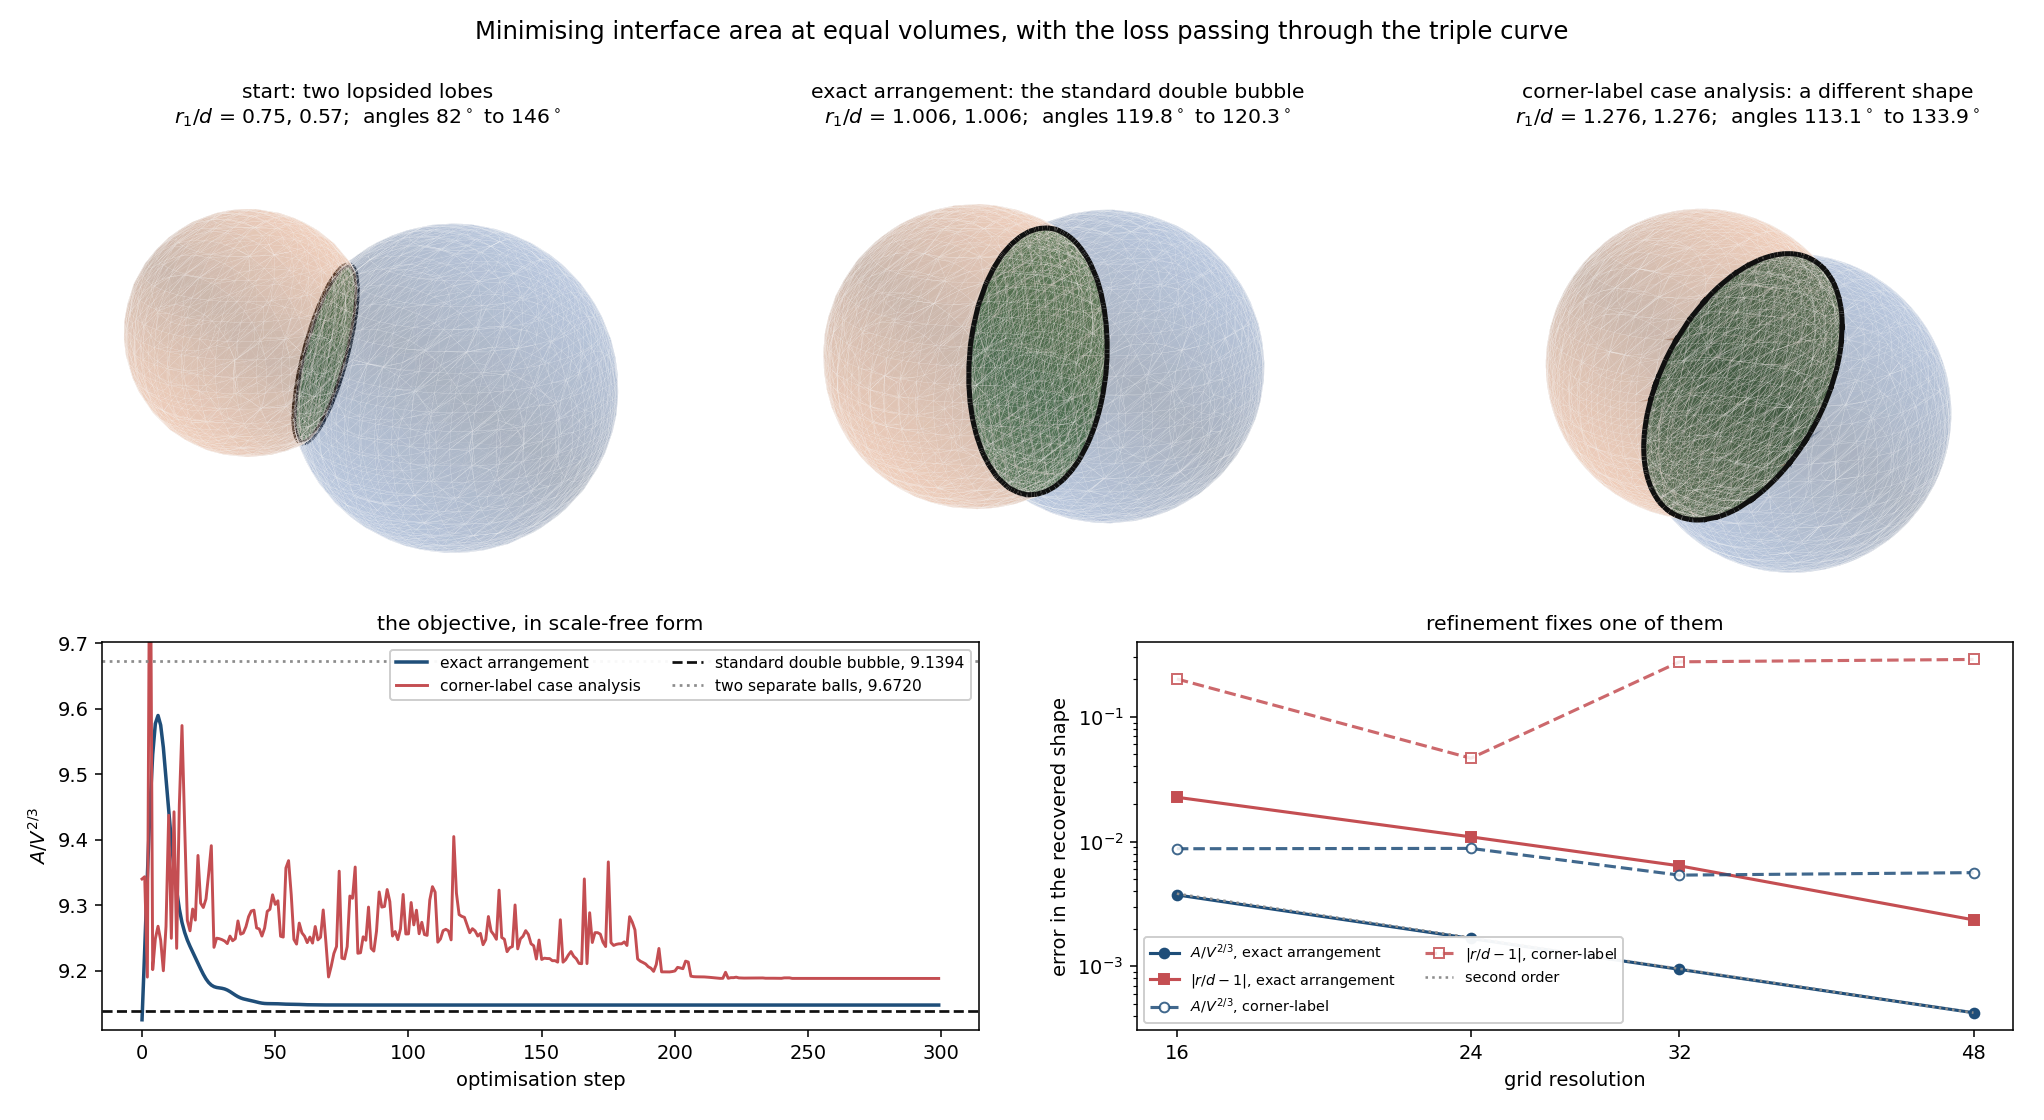
\includegraphics[width=0.80\linewidth]{double_bubble.png}
\caption{Minimising interface area at equal volumes in 3D. The loss is computed
on the extracted complex and differentiated back into the field, so every
gradient step passes through the triple curve (black). From the same lopsided
start (top left), the exact arrangement recovers the standard double bubble
(top centre) --- equal radii, a flat separating wall, dihedral angles within
$0.4^\circ$ of $120^\circ$ --- while substituting corner-label case analysis
and changing nothing else converges to a visibly different shape (top right).
Bottom left: our objective lands on the analytic minimum rather than on the
two-separate-balls configuration it has to beat, whereas the baseline settles
above it, jittering as it goes --- the jitter being its iterative solver rather
than the case analysis, which the ablation separates. Bottom right: our error
converges at second order, placing the residual in the discretisation rather
than the optimisation; the case analysis does not converge --- its shape error
is erratic and its objective error barely moves --- because its bias is
structural rather than a discretisation error.}
\label{fig:doublebubble}
\end{figure*}

\subsection{Contact between solid objects}
\label{sec:contact}

Section~\ref{sec:related} argued that composing one field per object and meshing
each independently loses the contact set. Objects here become channels of one
field, so interpenetration is not penalised but unrepresentable --- a point has
one argmax and therefore one owner --- and the surface two objects share is
emitted once, as a single set of triangles carrying their label pair. Two
questions follow: whether that surface is accurate, and whether it carries a
usable gradient. Everything below is run at a generic placement, since centring
the configurations would put the two-body patch and the three-body junction
curve on grid planes and grid lines at every even resolution, and measuring
there would measure a symmetry rather than the method.

Two balls of radius $r$ whose centres are $s$ apart put the contact patch on
their bisector plane as a disk of radius $\sqrt{r^2-s^2/4}$, with closed forms
for its area, that area's derivative and its rim; the rim is where both objects
and the background meet, so it is a triple curve of the partition and comes off
the same complex as the patch. Walking $s$ from deep overlap out to the loss of
contact, the area is accurate to $1.6\%$, its derivative to $0.7\%$ and the rim
to $0.7\%$ as long as the patch is more than five cells in radius, the errors
tracking that radius rather than the separation. The derivative is autograd
through the extraction rather than a difference quotient, and against a central
difference on the extractor itself it agrees to $1.5\times10^{-10}$ relative ---
the truncation error, not a discrepancy. Adding a third ball produces the
feature with no two-object analogue: at resolution $48$ the extractor returns
exactly two quadruple points, a count that is combinatorial and so is either
right or not, and the triple curve joining them has relative error
$3.7\times10^{-3}$. Refining from $24^3$ to $128^3$ gives fitted orders of
$1.99$ for the patch area and $1.97$ for that curve
(Figure~\ref{fig:contact}), so a piece of surface and the curve where three of
them meet converge alike. A patch interior is in fact reproduced exactly, since
$f_i-f_j$ is affine; the whole error is in where its boundary falls, which the
curved interfaces with the background set. The supplementary material tabulates the walk and the
three-object configuration in full.

That surface carries a usable gradient. Three objects start symmetric with equal
contact areas and a loss asks for three prescribed unequal ones, reading the
shared patches and nothing else --- no penalty term, no margin, no collision
query, because the partition cannot place two objects in the same spot to begin
with. After $140$ Adam steps on the centres and radii at $40^3$ the three areas
match their targets to $6.5\times10^{-5}$ relative error, worst of the three.
One boundary of this should be stated plainly. Beyond $s=2r$ there is no patch,
so its area and its gradient are both zero, while just inside onset the exact
derivative is $-\pi r$: the map from configuration to contact area is continuous
but not differentiable there, and the extractor reproduces that faithfully
rather than smoothing it. Gradients therefore maintain and reshape contact that
already exists; they do not pull separated objects into it. That is a property
of the quantity rather than of the extraction --- any objective posed on the
contact set has it --- and the usual remedy, an attraction term active within a
margin, is orthogonal to what is measured here.

\begin{figure*}[tbp]
\centering
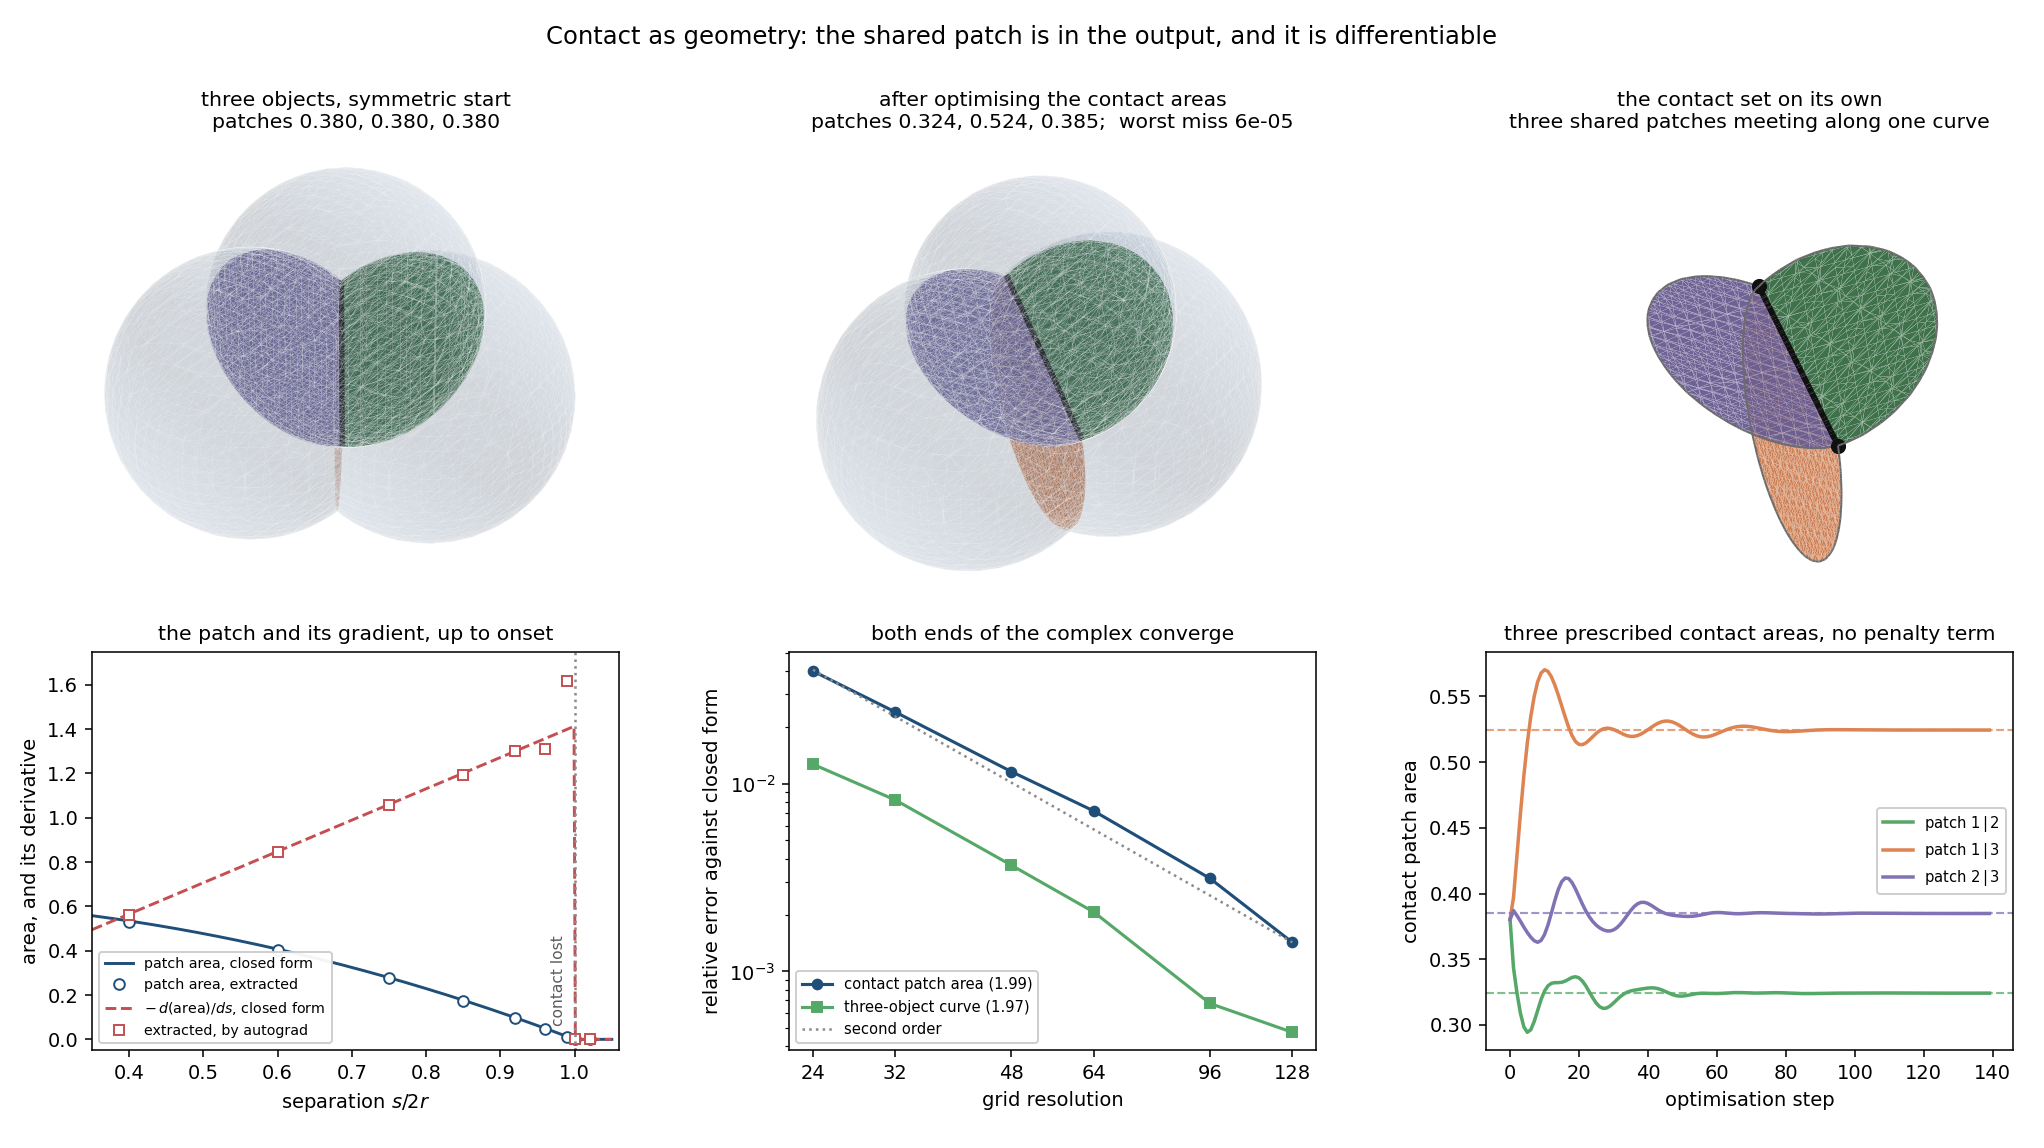
\includegraphics[width=0.80\linewidth]{contact.png}
\caption{Contact as geometry rather than as a penalty. Top: three objects
written as channels of one field, shown from a symmetric start and after
optimising their three contact areas to prescribed unequal values; the free
surfaces are translucent and the three shared patches opaque. Top right, the
contact set on its own --- three patches, each belonging to two objects at
once, closing onto the single curve (black) along which all three meet, which
terminates at the two quadruple points (dots) where the background joins them.
An independently meshed per-object representation produces the patches twice
and this curve not at all. Bottom left: patch area and its derivative against
closed form as the objects are walked apart, up to the separation at which
contact is lost and both fall to zero. Bottom centre: the patch area and the
three-object curve both converge at second order. Bottom right: the three
contact areas driven to their targets by a loss that reads nothing but the
shared patches, with no penalty term and no collision query, since the
partition cannot represent interpenetration in the first place.}
\label{fig:contact}
\end{figure*}

\subsection{A field nobody designed for us}
\label{sec:realdata}

Every field above is one we wrote down. To check that the construction survives
contact with data, we ran it on the per-class softmax volume of
TotalSegmentator's Couinaud liver-segment model~\cite{wasserthal2023} on a
thoracoabdominal CT. Eight segments tile one organ, so
segment--segment--segment curves are anatomy rather than contrivance. We took
the $49^3$ window containing the most cells with three or more distinct
labels --- $38.6 \times 38.6 \times 72$\,mm at the scan's native spacing, six
labels --- and placed the extraction grid so that its nodes coincide with voxel
centres, which they do to $2.1\times10^{-15}$, so the node values are the
network's own output and no resampling precedes the interpolation the method is
defined by. That the field holds probabilities rather than logits costs
nothing: softmax shifts every channel at a node by the same constant, which
cancels in every comparison the method makes. The partition being extracted is
exactly the model Hege et al.~\cite{hege1997} wrote down and then approximated
by $6^3$ subsampling.

On $663\,552$ tetrahedra the extractor returns $69\,211$ triangles carrying
$11$ distinct labelled interfaces, with $920$ triple-curve segments and $2$
quadruple points, in
$0.95$\,s (Figure~\ref{fig:realdata}a,b). Closure and orientation hold exactly; overshoot and residual are
identically zero, as exact solves against a per-cell affine interpolant
require, and the vertices lie
on the field's own interface to a median of $4.2\times10^{-16}$\,mm. Real data
needs the perturbation of Section~\ref{sec:degeneracy} more than our synthetic
fields did, because a quantised network output repeats values exactly across
voxels: at $\varepsilon = 0$ the positions are still bit-exact
($3.8\times10^{-15}$) but closure fails, and at $\varepsilon = 10^{-9}$ closure
holds with vertices displaced by
at most $5.3\times10^{-10}$\,mm, nine orders of magnitude below the voxel.

\paragraph{Against SurfaceNets.} The honest baseline is not per-label marching
cubes, a straw man against current tooling, but
\texttt{vtkSurfaceNets3D}~\cite{frisken2022, vtk}: a single multi-label pass,
threaded and fast, sharing points and cells between adjacent regions so no gaps
form, and in \texttt{vtkSurfaceNetsAtlas} organising its output into patches
keyed by ordered label pairs --- structurally the format of
Section~\ref{sec:assembly}. Two things separate it from what we do, and its own
documentation names both. It consumes an integer label map, so it cannot use the
sub-voxel interface position the field carries: measured against the same
interpolant, its vertices sit a median of $0.115$\,mm off, $0.14$ of a voxel,
rising to $1.19$ voxels at the $99$th percentile. And at locally non-manifold
configurations it duplicates points to keep the mesh manifold, after which, in
its words, ``duplicated points may diverge'' under smoothing. Identifying the
duplicates while coincident and reading their separation off the smoothed mesh
gives $18$ points in $6$ groups, ending a mean of $1.09$ and a maximum of
$1.32$ voxels apart (Figure~\ref{fig:realdata}c,d): the mesh tears by more than
a voxel exactly where three regions meet, whereas our triple-curve vertices are
single shared indices, so the same quantity is absent rather than small
(Proposition~\ref{prop:conform}). Judged against a yardstick neither method is
defined on --- the trilinear interpolant of the same probabilities, which is
Hege et al.'s model --- our vertices sit a median of $0.0095$ voxels from it on
the segment-to-segment walls against SurfaceNets' $0.090$, a gap that holds
into the tail.

None of this is an accuracy result: there is no ground truth for a clinical
segmentation, and every quantitative claim in this paper rests on the
closed-form fields above. The interface-distance comparison measures what
thresholding to integer labels discards, which is the point, and is not a
defect of SurfaceNets' implementation, since it never saw the probabilities.
The tearing is rare --- six sites in ten thousand points --- and is a statement
about the worst case at junctions rather than about the mesh on average.
The supplementary material gives
the per-vertex map and the full percentiles.


\begin{figure*}[tbp]
\centering
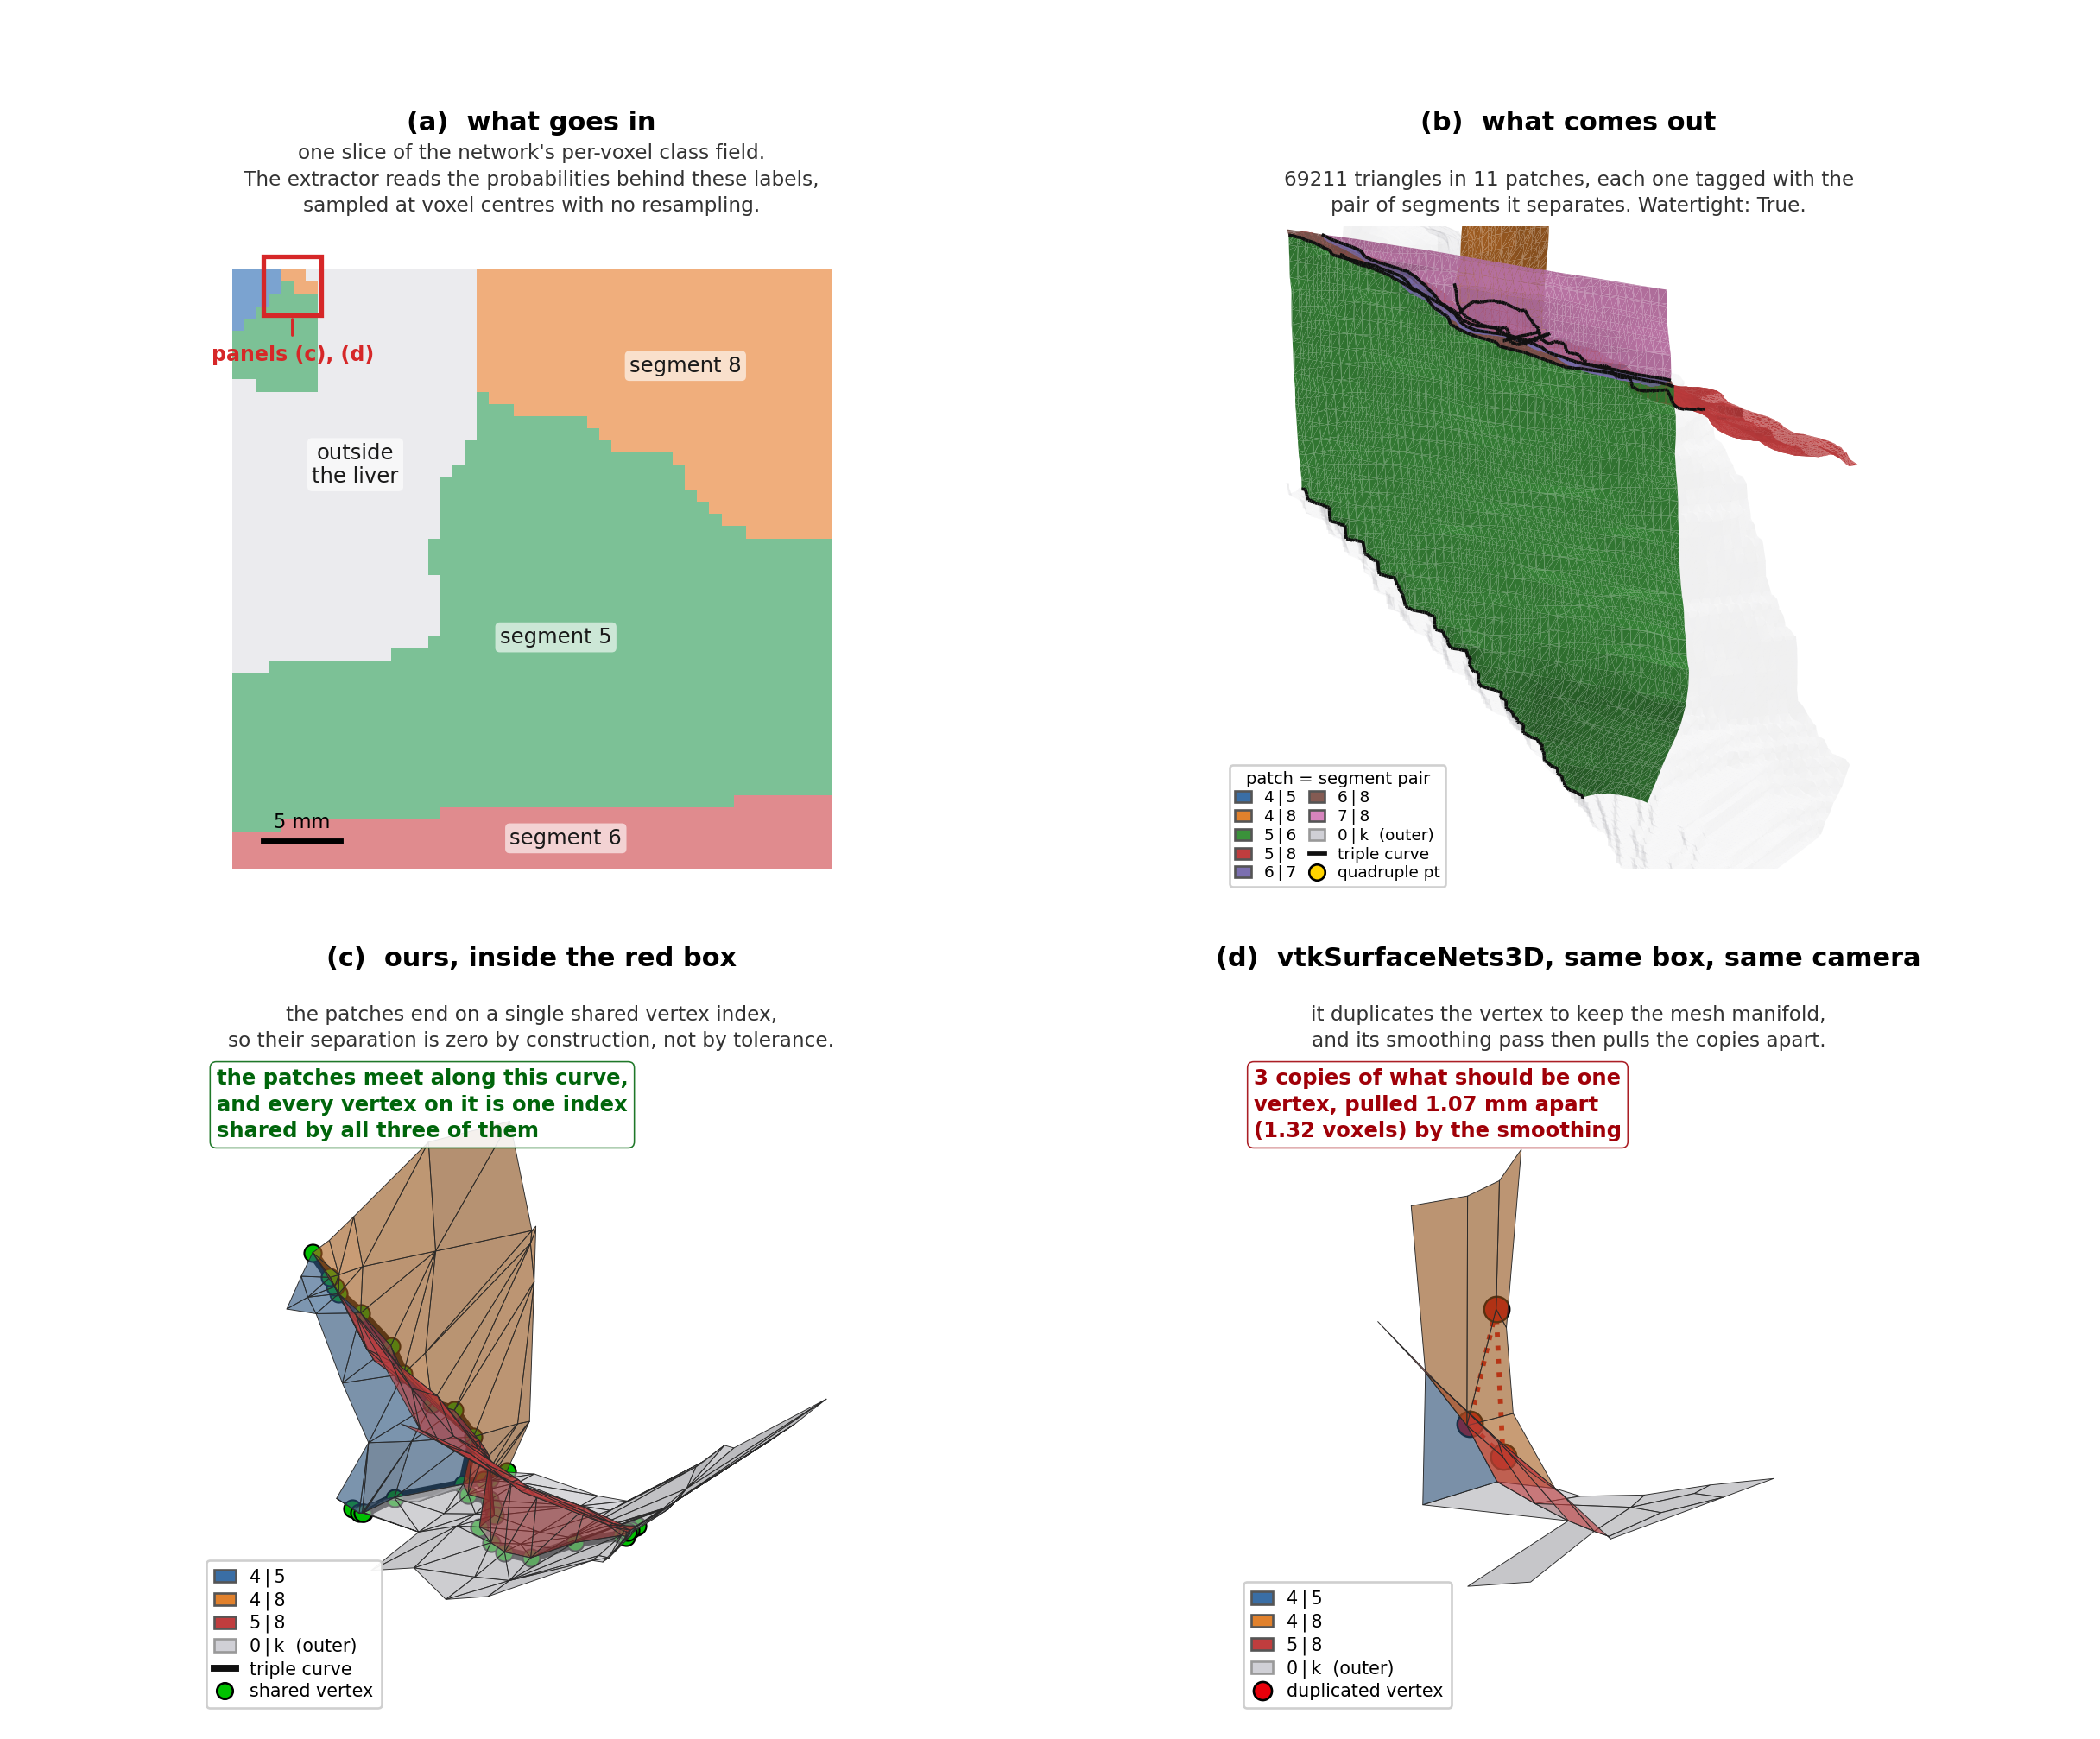
\includegraphics[width=0.70\linewidth]{realdata_liver.png}
\caption{Extraction from a segmentation network's probability volume on a
thoracoabdominal CT. (a) The input: one slice of the per-voxel class field,
with the red box marking the junction examined below. The extractor reads the
probabilities behind these labels, sampled at voxel centres. (b) The output:
every patch carries the pair of segments it separates, the outer boundary left
faint so the internal segment-to-segment walls are visible; these are the patches
no forward method tags separately. Triple curves are drawn in black. (c) and
(d) The boxed junction under both methods, same camera, same box, and coloured
by the same label-pair key --- SurfaceNets tags its cells with a label pair
exactly as we tag patches. Ours ends the three patches on one shared vertex
index; SurfaceNets duplicates the vertex to keep the mesh manifold, and its
smoothing pass then pulls the copies as far as $1.32$ voxels apart, the worst
of the six duplicated groups.}
\label{fig:realdata}
\end{figure*}

\subsection{The 2D instantiation}
\label{sec:2d}

The same construction in 2D --- crossings on edges of a triangular grid,
junctions inside triangles --- gives a self-contained extractor which passes
$24$ checks of its own. Among them is one the 3D studies cannot offer: the
\emph{Jacobian} of a triple point with respect to the sites matches the
analytic derivative of the circumcentre to $2.9\times10^{-16}$, which is a
stronger statement than finite-difference agreement because it compares against
a formula rather than against another numerical path.

We use it for the optimisation studies that need many cheap iterations.
Matching a target partition with a randomly initialised neural field reduces
the loss by $98.9\%$ in $260$ steps. Minimising interface length under
equal-area constraints on a disk, where the analytic minimiser is the
three-fold $120^\circ$ configuration of length $3R$, reaches $2.4000$ against
the exact $2.40$ for a power-diagram field; the same objective on a neural field
improves the length but stalls at $114.5^\circ, 114.6^\circ, 130.9^\circ$. The
extractor is identical in both runs, so that gap reflects the optimisation
landscape of the over-parameterised representation rather than the extraction,
and we report it as a negative result rather than tuning it away. Details and
figures are in the supplementary material.
\section{Limitations}
\label{sec:limitations}

\paragraph{Assumptions and accuracy.} The one assumption remaining is that a
label occupying a cell also reaches that cell's boundary, so a region small
enough to lie strictly inside a single tetrahedron is invisible. Unlike the
failure it replaces this is a genuine resolution condition that refinement
removes, and it is screened for rather than assumed away: the implementation
samples each tetrahedron's interior at five points and reports any label
winning there that the enumeration never saw, and no field reported here
produced one. Five samples is a screen and not a decision procedure, so that
bounds the condition on the fields we ran rather than excluding it. Accuracy on
curved interfaces is likewise limited by the $P_1$ interpolation of the logits
rather than by the extraction; keeping the exact arrangement for the
combinatorial structure and projecting each vertex onto the true field by a few
Newton steps would decouple accuracy from differentiability. Reproducing the
argmax partition exactly is also not the same as reproducing prescribed region
volumes, which volume-fraction reconstruction requires, and the natural route
to it here --- fitting the node logits by descent on volume error --- is
untested.

\paragraph{Degeneracy is handled by perturbation, not exactly.}
Section~\ref{sec:degeneracy} trades an $O(\varepsilon)$ position error for
genericity; an exact treatment would have to admit vertices at grid nodes and
shared triple points as first-class entities. This is the weaker half of the
exchange made against Du et al.~\cite{du2022}, whose exact predicates decide
those configurations correctly instead of perturbing them away.
Sections~\ref{sec:further} and~\ref{sec:headtohead} bound the concession
without removing it, but they are evidence rather than proof: their guarantee
covers every input, ours is agreement on a finite sample we constructed. We
have also not compared on the very large scenes where their lookup table earns
its cost. What the perturbation buys is a vertex that has coordinates at all,
which is what a gradient needs.

\paragraph{Optimisation is demonstrated, not surveyed.} Both minimal-interface
studies place the minimiser inside the field family by construction, so what
they exercise is the gradient path through the non-manifold features rather
than descent on a representation not fitted to the answer. The 2D neural-field
run of Section~\ref{sec:2d} stalls short of its minimiser, and we have not
characterised when that difference bites. Nor are we free of initialisation
dependence: of five starts for the double bubble, four recover it and the most
lopsided lets the lobes come apart into two balls, after which there is no
shared wall to pull them back --- the descent failing rather than the
extractor, whose output stays watertight, but a failure. Where a two-label
optimisation can be compared against a method built for it,
Section~\ref{sec:flexicubes} puts us behind: FlexiCubes settles five times
closer to the target at an indistinguishable objective value, because averaging
a cell's crossings into one dual vertex damps field noise that we report
faithfully. At $K=2$ that is a reason to prefer theirs; what the construction
offers is the case $K>2$, which theirs cannot express. Contact gradients have a
boundary of their own: there is no derivative with respect to a configuration
in which the objects are apart, so the operator reshapes contact that already
exists rather than finding it, and pairing it with an attraction term active
within a margin is the obvious untested remedy.

\paragraph{Scope.} We extract interfaces, not volume meshes. Feeding the output
to an unfitted or body-fitted solver, the motivating application for
multi-material CAE~\cite{fromm2025, nife2024}, is future work --- as is the
cardiac pipeline of Section~\ref{sec:intro}, for which we have established that
the operator fits the input contract but have not run the fibre computation.
Section~\ref{sec:realdata} demonstrates the extraction on clinical segmentation
output, but on liver segments rather than cardiac chambers, because the
cardiac-chamber model of the same toolkit is not openly licensed; nothing in the
method distinguishes the two cases.

\section{Conclusion}

The exact arrangement of a piecewise-linear multi-label field is not the open
part: it is computed, and computed robustly, by exact-predicate
methods~\cite{du2022}. What those methods cannot do is hand a gradient back,
because the implicit vertex encoding that makes them robust leaves nothing to
differentiate. The differentiable extractors have the converse problem: asked
for three regions, the strongest of them must be run once per region, and its
cell-averaged vertices then round the shared wall differently from each side,
leaving three percent of the domain claimed twice or not at all at every
resolution we tried (Section~\ref{sec:flexicubes}). Obtaining the same
arrangement from explicit closed-form linear solves --- rather than reading a
cell's interface off its corner labels, which we show is wrong for roughly half
of three-label faces in 3D at a rate refinement does not improve --- closes
that gap, and the remaining difficulties dissolve with it. Patches become
convex, so triangulation cannot fold; vertices become small linear solves, so
ordinary automatic differentiation suffices; and cells agree across shared
faces automatically, so nothing needs welding. What that buys is visible in the
setting the partition was always implicitly about. Writing several objects as
channels of one field makes interpenetration unrepresentable rather than merely
penalised, and the exact arrangement returns the contact between them as
geometry: one shared patch instead of two coincident sheets, bounded by triple
curves that are themselves in the output, all of it differentiable. A loss
written on nothing but the contact set is enough to place it.

\section*{Acknowledgements}

\noindent The clinical example rests entirely on openly released work: both the
Couinaud liver-segment model and the example CT it runs on come from
TotalSegmentator~\cite{wasserthal2023}. Neither comparison would have been
possible without released implementations --- Du et al.~\cite{du2022} for
Section~\ref{sec:headtohead}, Shen et al.~\cite{shen2023} for
Section~\ref{sec:flexicubes} --- and both were run against their authors' code
rather than a reimplementation.

\paragraph*{Code and data.} The extractor, the automated checks, the
experiment scripts, and the harnesses that build and drive the reference
implementations of Du et al.~\cite{du2022} and FlexiCubes~\cite{shen2023} are
public at
\url{https://github.com/aiscienceresearch/differentiable-multi-material-interfaces},
together with the numerical results behind every table and figure. The clinical
probability volume is not redistributed; a script fetches it from its source.

\paragraph*{Use of generative AI.} In accordance with the Eurographics policy,
this work used a commercial large language model assistant during preparation:
drafting and revising prose, restructuring the manuscript, assisting with the
implementation and with running the validation and figure scripts, and
searching the literature. The research questions, the formulation, the method
and the interpretation of the results are the author's, who reviewed all
generated text, code and numbers and takes full responsibility for the entire
content of the article; every quantitative claim is reproducible from the
released code.

\bibliographystyle{eg-alpha-doi}
\bibliography{refs}

\end{document}
